% CVPR 2022 Paper Template
% based on the CVPR template provided by Ming-Ming Cheng (https://github.com/MCG-NKU/CVPR_Template)
% modified and extended by Stefan Roth (stefan.roth@NOSPAMtu-darmstadt.de)

\documentclass[10pt,twocolumn,letterpaper]{article}

%%%%%%%%% PAPER TYPE  - PLEASE UPDATE FOR FINAL VERSION
\usepackage[review]{cvpr}      % To produce the REVIEW version
%\usepackage{cvpr}              % To produce the CAMERA-READY version
%\usepackage[pagenumbers]{cvpr} % To force page numbers, e.g. for an arXiv version

% Include other packages here, before hyperref.
\usepackage{graphicx}
\usepackage{threeparttable}
\usepackage{amsmath}
\usepackage{amssymb}
\usepackage{booktabs}
\usepackage{multirow}
\usepackage{enumitem}
\usepackage{bm}
\usepackage{xcolor}
\usepackage{color, colortbl}
\newcommand{\lsh}[1]{\textcolor{magenta}{ (lsh: #1)}}
\newcommand{\tablestyle}[2]{\setlength{\tabcolsep}{#1}\renewcommand{\arraystretch}{#2}\centering\footnotesize}
\newlength\savewidth\newcommand\shline{\noalign{\global\savewidth\arrayrulewidth
  \global\arrayrulewidth 1pt}\hline\noalign{\global\arrayrulewidth\savewidth}}
% \newcommand{\myplus}[1]{\color{green}{\tiny{$+$#1}}}
% \newcommand{\myminus}[1]{\color{red}{\tiny{$-$#1}}}
\newcommand{\myplus}[1]{\color{green}{\tiny{}}}
\newcommand{\myminus}[1]{\color{red}{\tiny{}}}
\newcommand{\xd}[1]{\color{orange}{\tiny{$-$}#1}}

\newcommand\mypara[1]{\vspace{1mm}\noindent\textbf{#1}}

% It is strongly recommended to use hyperref, especially for the review version.
% hyperref with option pagebackref eases the reviewers' job.
% Please disable hyperref *only* if you encounter grave issues, e.g. with the
% file validation for the camera-ready version.
%
% If you comment hyperref and then uncomment it, you should delete
% ReviewTempalte.aux before re-running LaTeX.
% (Or just hit 'q' on the first LaTeX run, let it finish, and you
%  should be clear).
\usepackage[pagebackref,breaklinks,colorlinks]{hyperref}


% Support for easy cross-referencing
\usepackage[capitalize]{cleveref}
\crefname{section}{Sec.}{Secs.}
\Crefname{section}{Section}{Sections}
\Crefname{table}{Table}{Tables}
\crefname{table}{Tab.}{Tabs.}


%%%%%%%%% PAPER ID  - PLEASE UPDATE
\def\cvprPaperID{7432} % *** Enter the CVPR Paper ID here
\def\confName{ICCV}
\def\confYear{2022}


\newcommand{\ky}[1]{{\color{blue}{#1}}}
\newcommand{\KY}[1]{{\color{blue}{\bf #1}}}

% \newcommand{\sf}[1]{{\color{red}{#1}}}
\newcommand{\SF}[1]{{\color{red}{\bf #1}}}

\begin{document}

%%%%%%%%% TITLE - PLEASE UPDATE
%\title{Self-assembling Knowledge Distillation via Semantic Position Encoding}

\title{TiG-BEV: Multi-view BEV 3D Object Detection via\\Target Inner-Geometry Learning}

%\title{Self-assembling Knowledge Distillation with Semantic Alignment}

\author{First Author\\
Institution1\\
Institution1 address\\
{\tt\small firstauthor@i1.org}
% For a paper whose authors are all at the same institution,
% omit the following lines up until the closing ``}''.
% Additional authors and addresses can be added with ``\and'',
% just like the second author.
% To save space, use either the email address or home page, not both
\and
Second Author\\
Institution2\\
First line of institution2 address\\
{\tt\small secondauthor@i2.org}
}
\maketitle

\begin{abstract}
As a popular paradigm for juggling data privacy and collaborative training, federated learning~(FL) is flourishing to distributively process the large scale of heterogeneous datasets on edged clients. Due to bandwidth limitations and security considerations, it ingeniously splits the original problem into multiple subproblems to be solved in parallel, which empowers \textit{primal dual} solutions to great application values in FL. In this paper, we review the recent development of classical \textit{federated primal dual} methods and point out a serious common defect of such methods in non-convex scenarios, which we say is a ``dual drift'' caused by dual hysteresis of those longstanding inactive clients under partial participation training. To further address this problem, we propose a novel \textit{\textbf{A}ligned \textbf{Fed}erated \textbf{P}rimal \textbf{D}ual}~(\textit{\textbf{A-FedPD}}) method, which constructs virtual dual updates to align global consensus and local dual variables for those protracted unparticipated local clients. Meanwhile, we provide a comprehensive analysis of the optimization and generalization efficiency for the \textit{A-FedPD} method on smooth non-convex objectives, which confirms its high efficiency and practicality. Extensive experiments are conducted on several classical FL setups to validate the effectiveness of our proposed method. 
\end{abstract}
\section{Introduction}\label{sec:intro}
% Multi-armed bandit (MAB) is a classic sequential decision making problem \citep{auer2002finite}, where a learning agent chooses among competing actions sequentially to maximize its accumulative reward over time. 
% %Despite its simplicity, MAB exemplifies the exploration-and-exploitation dilemma that also exists in more complicated problems. 
% An important extension of MAB, named linear contextual bandit \citep{li2010contextual}, incorporates contextual information in the problem setting, by assuming a linear mapping between the context and expected reward. It has gained popularity in various applications, such as recommender systems \citep{li2010contextual}, display advertisement \citep{li2010exploitation} and clinical trials \citep{durand2018contextual}.
% Most existing linear bandit solutions are designed under a centralized learning setting, i.e., data is readily available at a central server. However, with the increasing public concerns of privacy, especially the bandit algorithms usually directly learn from user data,
% %more and more people are reluctant to provide their own data and strict regulations on data usage like GDPR have also went into effect \cite{voigt2017eu}, which makes 
% there is a growing demand to keep data decentralized and push the learning of bandit models to the client side. 
% % This idea is also made much more feasible due to the growing computational power of edge devices nowadays. 

% Federated learning has recently emerged as a promising setting for decentralized machine learning.
% % , and its effectiveness was first validated at a large scale by training a global model across all mobile devices via the Google Keyboard Android application \cite{konevcny2016federated}. 
% %The term ``federated learning" was first introduced by \citet{mcmahan2017communication} with an emphasis on efficiently training deep models over mobile device applications. As significant amount of later works have applied federated learning to other applications, there may be variations in its meaning for different research communities. 
% Since its debut in \citet{mcmahan2017communication}, there have been variations in its definition for different applications \citep{yang2019federated}.
% In this paper, we follow the general definition by \citet{kairouz2019advances}: multiple clients collaborate in solving a machine learning problem under the coordination of a central server, while keeping each client's raw data local. 
% So far, most existing works in federated learning study offline supervised learning problems \citep{konevcny2016federated,zhao2018federated}, where labeled training instances already sit on the client side. How to perform bandit learning under the federated learning setting remains underexplored.
As a popular online learning problem, linear contextual bandit has been used for a variety of applications, including recommender systems \citep{li2010contextual}, display advertisement \citep{li2010exploitation} and clinical trials \citep{durand2018contextual}. While most existing solutions are designed under a centralized setting (i.e., data is readily available at a central server), in response to the increasing application scale and public concerns of privacy, there is a growing demand to keep data decentralized and push the learning of bandit models to the client side.
% As a classic sequential decision making problem, linear contextual bandit has been widely used for a variety of real-world applications, including recommender systems \citep{li2010contextual}, display advertisement \citep{li2010exploitation} and clinical trials \citep{durand2018contextual}. 
% Most existing solutions are designed under a centralized learning setting, i.e., data is readily available at a central server. However, with the increasing public concerns of privacy, especially the bandit algorithms usually directly learn from user data,
% there is a growing demand to keep data decentralized and push the learning of bandit models to the client side. 
Federated learning has recently emerged as a promising setting for decentralized machine learning \citep{konevcny2016federated}.
% , and its effectiveness was first validated at a large scale by training a global model across all mobile devices via the Google Keyboard Android application \cite{konevcny2016federated}. 
%The term ``federated learning" was first introduced by \citet{mcmahan2017communication} with an emphasis on efficiently training deep models over mobile device applications. As significant amount of later works have applied federated learning to other applications, there may be variations in its meaning for different research communities. 
Since its debut in \citeyear{mcmahan2017communication}, there have been many variations for different applications \citep{yang2019federated}. However, most existing works study offline supervised learning problems \citep{li2019convergence,zhao2018federated}, which only concerns optimization convergence over a fixed dataset. How to perform federated bandit learning remains under-explored, and is the main focus of this paper. 

Analogous to its offline counterpart, the goal of federated bandit learning is to minimize the cumulative regret incurred by $N$ clients during their online interactions with the environment over time horizon $T$,
% $N$ clients in a learning system need to collaborate to minimize the overall cumulative regret over a finite time horizon $T$, 
while keeping each client's raw data local. Take recommender systems as an example, where the clients correspond to the edge devices that directly interact with user by making recommendations and receiving feedbacks. Unlike centralized setting where observations from all clients are immediately transmitted to the server to learn a single model, in federated bandit learning, each client makes recommendations based on its local model, with occasional communication for collaborative model estimation.

% In this paper, we follow the general definition by \citet{kairouz2019advances}: multiple clients collaborate in solving a machine learning problem under the coordination of a central server, while keeping each client's raw data local. 


%Though having potential for wide range of applications, online learning problems like linear bandit in federated learning setting, a.k.a. federated linear bandits \cite{dubey2020differentially}, have not attracted enough attention and still remain an open problem. 

% Therefore, it is a natural idea to study contextual linear bandit in a federated learning paradigm, which is also referred to as federated linear bandits \cite{dubey2020differentially}. In a federated learning paradigm, multiple clients collaborate in solving a machine learning problem, under the coordination of a central server, and each client's raw data is stored locally and not transferred to the server. 
% when linear bandit algorithms are applied to the federated learning paradigm, because these algorithms assume a traditional centralized machine learning system where all the data are collected together and all the computation happens in one machine or data center. 
Several new challenges arise in this problem setting. 
The first is the conflict between the need of timely data/model aggregation for \emph{regret minimization} and the need of \emph{communication efficiency}, since communication is the main bottleneck for many distributed application scenarios, e.g., communication in a network of mobile devices can be slower than local computation by several orders of magnitude \citep{huang2013depth}. A well-designed communication strategy becomes vital to strike the balance. 
In addition, 
% constraints from real-world applications should also be taken into consideration when designing the communication strategy. For example, 
the clients often have various response time and even occasional unavailability in reality, due to the differences in their computational and communication capacities.
% the clients may differ in their computational and communication capacities. This will lead to various response time and even occasional unavailability. 
This hampers global synchronization employed in existing federated bandit solutions \citep{wang2019distributed,dubey2020differentially}, which requires the server to first send a synchronization signal to all clients, wait and collect their returned local updates, and finally send the aggregated update back to every client.
Second, it is very restrictive to only assume homogeneous clients, i.e., they solve the same learning problem. 
% As bandit algorithms are mostly deployed to interact with individual users, studying heterogeneous clients with personalized learning problems has a greater potential.
Studying \emph{heterogeneous clients} with distinct learning problems has a greater potential in practice.
This is referred to as ``\emph{non-IIDness}" of data in the context of federated learning, e.g., the difference in $\mathcal{P}_{i}(\bx,y)=\mathcal{P}_{i}(\bx) \mathcal{P}_{i}(y|\bx)$ is caused by each client $i\in[N]$ serving a particular user or group of users, a particular geographic region, or a particular time period. Apparently, it is also unreasonable to assume every client has equal amount of new observations, which however is assumed in existing works. 

%To be more concrete, due to the time-varying arm set $\cA_{t}$ and the dependence on history data for arm selection in linear bandit, context vector $X$ is non-IID in nature and is not the main concern. 
% It is not a major concern since the performance metric, i.e. regret $r_{t}$, is defined against the best arm in $\cA_{t}$. 

% For example, internet connection and the different computation power of devices.
% \textcolor{red}{reasons we need async algo}

% This naturally leads to the question: how to balance between regret minimization and communication efficiency in the federated linear bandit problem.
To address the first challenge, we propose an asynchronous event-triggered communication framework for federated linear bandit. 
%Our event-triggering mechanism offers a flexible way to balance between the regret-minimization and communication-efficiency dilemma. 
Communication with a client happens only when the last communicated update to the client becomes irrelevant to the latest one; and we prove only by then effective regret reduction can be expected in this client because of the communication. 
Under this asynchronous communication, each client sends local update to and receives aggregated update from the server independently from other clients, with no need for global synchronization. This improves our method's robustness against possible delays and temporary unavailability of clients. It also brings in reduced communication cost when the clients have distinct availability of new observations, because global synchronization requires every client in the learning system to send its local update despite the fact that some clients can have very few new observations since last synchronization.
% make the proposed method more robust and practical against the infrastructure constraints, because the aggregated update sent to each client is asynchronous and  
% This makes our method more robust against possible delays in the communication, and we prove that the client enjoys the same benefit in regret reduction as long as it receives the update before its next interaction with the environment.

To address the second challenge, we design algorithms for federated linear bandit with both ``\emph{IIDness}" and ``\emph{non-IIDness}" based on the proposed communication framework. We consider two different assumptions on the reward functions. First, all the clients share a common reward function i.e., a single model is learned for all clients. Second, each client has a distinct reward function with mutual dependence captured by globally shared components in the unknown parameter, which resembles 
%so one model per client is learned during the interaction with the environment, which in essence is similar to the problem considered in
federated multi-task learning \citep{smith2017federated}.
We rigorously prove the upper bounds of accumulative regret and communication cost for the proposed algorithms in these two settings, and conduct extensive empirical evaluations to demonstrate the effectiveness of our proposed framework.
% especially its flexibility in balancing the trade-off between regret and communication cost.


\section{Related Works}
\paragraph{Camera-based 3D Object Detection.} Camera-based 3D object detection has been widely used for applications like autonomous driving since its low cost compared with LiDAR-based detectors. FCOS3D \cite{b12} first predicts the 3D attributes of objects through the features around 2D centers and PGD \cite{b17} utilizes the relational graphs to improve the depth estimation for 3D monocular object detection. Further, MonoDETR~\cite{b47} introduces DETR-like~\cite{b18} architectures without complex post-processing.
Recently, Bird’s-Eye-View~(BEV), as a unified representation of surrounding views same as LiDAR-based detector, has attracted much attention. DETR3D \cite{b13} follows the DETR \cite{b18} to adopt the 3D reference points in BEV space by using object queries. BEVDet \cite{b19} utilizes the Lift-Splat-Shoot~(LSS) operation \cite{b20} to transform 2D image features into 3D Ego-car coordinate to generate 3D BEV feature. PETR \cite{b21} obtain the 3D position-aware ability by 3D positional embedding. Inspired by the recently developed attention mechanism, BEVFormer \cite{b11} and PolarFormer \cite{b22} automates the camera-to-BEV process with learnable attention modules and queries a BEV feature according to its position in 3D space. To further improve the detection performance, the temporal information has been introduced in BEVDet4D \cite{b23} and PETRv2 \cite{b24}, which achieve significant performance enhancement. Moreover, BEVDepth \cite{b7} observes that accurate depth estimation is essential for BEV 3D object detection supervised by projected LiDAR points. MonoDETR-MV~\cite{b48} proposes a depth-guided transformer for multi-view geometric cues, but predicts only foreground depth map without dense depth supervision. As a LiDAR-to-camera learning scehme, our TiG-BEV leverages the pre-trained LiDAR-based detector to improve the performance of camera-based detectors for multi-view BEV 3D object detection.

\paragraph{Depth Estimation.} Depth estimation is a classical problem in computer vision. These method can be divided into single-view depth estimation and multi-view depth estimation. Single-view depth estimation is either regarded as a regression problem of a dense depth map or a classification problem of the depth distribution. \cite{b26, b27, b28, b29, b30} generally build an encoder-decoder architecture to regress the depth map from contextual features. Multi-view depth estimation methods usually construct a cost volume to regress disparities based on photometric consistency \cite{b31, b32, b33, b34, b35, b62}. For 3D object detection, previous methods~\cite{b61,b51,b52} also introduce additional networks for depth estimation to improve the localization accuracy in 3D space.
Notably, MonoDETR \cite{b47,b48} proposes to only predict the foreground depth maps instead of the dense depth values, but cannot leverage the advanced geometries provided by LiDAR modality. Different from them, our TiG-BEV conducts inner-depth supervision that captures local sptial structures of different foreground targets.

\paragraph{Knowledge Distillation.} Knowledge Distillation has shown very promising ability in transferring learned representation from the larger model (teacher) to the smaller one (student). Prior works \cite{b37, b38, b39, b40} have been proposed to help the student network learn the structural representation for better generalization ability. These methods generally utilize the correlation of the instances to describe the geometry, similarity, or dissimilarity in the feature space. The following methods extend the teacher-student paradigm to many vision task, demonstrating its effectiveness including action recognition \cite{b41}, video caption \cite{b42}, 3D representation learning~\cite{b59,b49,b50,b60}, object detection \cite{b43, b44} and semantic segmentation \cite{b45, b46}. However, only a few of works consider the multi-modal setting between different sensor sources. For 3D representation learning, I2P-MAE~\cite{b49} leverages masked autoencoders to distill 2D pre-trained knowledge into 3D transformers. UVTR \cite{b25} presents a simple approach by directly regularizing the voxel representations between the student and teacher models. BEVDistill \cite{b9} transfer knowledge from LiDAR feature to the cam feature by dense feature distillation and sparse instance distillation. Our TiG-BEV also follows such teacher-student paradigm and effectively distills knowledge from the LiDAR modality into the camera modality,


%However, they overestimated the prior of spatial order while neglected the issues of semantic mismatch, \ie, the pixels of teacher feature map often contains richer semantic compared to that of student on the same spatial location. We found that some works~\cite{Park2019RelationalKD, Passalis2018LearningDR,Peng2019CorrelationCF,Tung2019SimilarityPreservingKD,Yim2017AGF,huang2017like,Liu2021ICKD}, though unintended, have been proposed to relax the spatial constrain during feature transfer. Typically, they defined the relational graph, and similarity matrix in the feature space of teacher network and transferred it to the student network. For instances, Tung and Mori~\cite{Tung2019SimilarityPreservingKD} calculated the similarity matrix where each entry encoded the similarity between two instances. Liu \etal~\cite{Liu2021ICKD} measured the correlation between channels by inner-product. They condensed and compressed the entire feature to some properties (often scalar) and thus collapsed the spatial information. On the other hand, such process damaged the original teacher feature and may lead to sub-optimal solution. 

%The spread of KD has also driven some methods designed for specific vision tasks including video captioning~\cite{pan2020spatio}, action recognition~\cite{wang2019progressive,cui2020knowledge}, object detection~\cite{chen2017learning,zhang2020improve,dai2021general} and semantic segmentation~\cite{liu2019structured,he2019knowledge,Wang2020IntraclassFV}. Regarding the semantic segmentation, these methods are indeed related to relation knowledge distillation which computes similarity matrix~\cite{Tung2019SimilarityPreservingKD}. To investigate the potential of our method, we also adapt the method to semantic segmentation with hierarchical distillation.




% \begin{figure*}[t]
%   \centering
%   \includegraphics[width=\textwidth]{cvpr_2022/framework_4.pdf}
%   \vspace{-5mm}
%   \caption{Illustration of our framework. (a) \textbf{Target-aware Transformer}. Conditioned on the teacher feature and the student feature, the transformation map Corre. is computed and then applied on the student feature to reconfigure itself, which is then asked to minimize the L$_2$ loss with the corresponding teacher feature. (b) \textbf{Patch-group Distillation}. Both teacher and student features are to be sliced and rearranged as groups for distillation. By concatenating the patches within a group, we explicitly introduce the spatial correlation among the patches beyond the patches themselves. (c) \textbf{Anchor-point Distillation}. Each color indicates a region. We use average pooling to extract the \textit{anchor} within a local area of the given feature map, forming the new feature map of a smaller size. The generated anchor-point features will participate in the distillation.}
%   \label{fig:framework}
%   \vspace{-5mm}
% \end{figure*}

%-------------------------------------------------------------------------
%\usepackage{amsmath}
%\usepackage{autobreak}
\section{Method}
\label{sec:method}
% There is a temptation, though, to let the student perfectly mimic the teacher, which does not appear to be viable in reality because student is inferior to teacher in learning capacities. Rather, we introduce the cross-attention to assist the feature matching between student and teacher. The cross-attention is conditioned by a pair of teacher feature and student feature that reflects the context of two given features. In practice \cite{Cho2019OnTE,Ji2021ShowAA,Chen2020CrossLayerDW}, it's hard for the student to directly match (\ie reconstruct) a teacher layer. Prior methods used an attention \textit{weight} to regulate the loss function or decide the allocation of the teacher layers to student, which is a global manner. In contrast, our method allows the student to perform self-assessment through the cross-attention and be aware of the difference and similarity compared to teacher feature, which can facilitate the knowledge transfer. (See Figure~\ref{fig:framework} (a)).


% In this section, we will provide a detailed description of the proposed cross-modality distillation method. The overall architecture is illustrated by Fig. 1. Our architecture consists of three branch: Lidar-based detector branch, Multi-view based detector branch and the cross-modal supervision. We will introduce cross-modal supervision components in detail in the following sections. 

\begin{figure*}[t!]
  \centering
  % \vspace{0.2cm}
  \includegraphics[width=\textwidth]{cvpr_2022/iccv_fig4.drawio.png}
  % \vspace{-5mm}
  \caption{\textbf{Overall Framework of TiG-BEV,} which contains a pre-trained LiDAR-based detector as teacher, a camera-based detector as student, and a target inner-geometry scheme for cross-model learning. Our proposed learning paradigm effectively transfers the inner-geometry semantics of the LiDAR modality via two components, an inner-depth supervision (Section~\ref{sec:Inner-depth Supervision}) for foreground relative depth, and an inner-feature BEV distillation (Section~\ref{sec:Inner-feature BEV Distillation}) from both channel-wise and keypoint-wise.}
  \label{fig:framework}
  % \vspace{0.3cm}
  % \vspace{-5mm}
\end{figure*}

The overall architecture of TiG-BEV is shown in Figure~\ref{fig:framework}, which consists of three components: the student camera-based detector, the teacher LiDAR-based detector, and our proposed target inner-geometry learning scheme. In Section~\ref{sec:Baseline Models}, we first introduce the adopted baseline models. Then, we specifically illustrate the designs of TiG-BEV for inner-depth supervision in Section~\ref{sec:Inner-depth Supervision} and inner-BEV feature distillation in Section~\ref{sec:Inner-feature BEV Distillation}. Finally in Section~\ref{sec:overall_loss}, we present the overall loss of our TiG-BEV for LiDAR-to-camera learning.

\subsection{Baseline Models}
\label{sec:Baseline Models}
\paragraph{Student Camera-based Detector.}
By default, we adopt BEVDepth~\cite{b7} as our student camera-based detector for multi-view 3D object detection. 
Given the input multi-view images (normally 6 views for a scene), the student model first utilizes a shared 2D backbone and FPN module~\cite{b54} to extract the $C$-channel visual features $\{F_i\}_{i=1}^6$, where $F_i \in {\mathbb{R}^{C\times H_v\times W_v}}$, and $H_v, W_v$ denote the size of feature maps. These features are fed into a shared depth network to generate the categorical depth map~\cite{b51}, $\{D_i\}_{i=1}^6$, where ${D_i}\in {\mathbb{R}^{D\times H_v\times W_v}}$, where D denotes the pre-defined number of depth bins. During training, BEVDepth adopts dense depth supervision for the predicted depth maps, which projects the paired LiDAR input onto multi-view image planes to construct pixel-by-pixel absolute depth ground truth, $\{D_i^{gt}\}_{i=1}^6$, where ${D_i^{gt}}\in {\mathbb{R}^{1\times H_v\times W_v}}$. 
Then, following~\cite{b20}, the multi-view visual features are projected into a unified BEV representation via the predicted depth maps, which is further encoded by a BEV encoder, denoted as $F^{2d}_{\rm bev}\in {\mathbb{R}^{C\times H_{\rm bev}\times W_{\rm bev}}}$. Finally, the detection heads are applied on top to predict objects in 3D space. We represent the two basic losses of the student model as $\mathcal{L}_{\rm{depth}}^{A}$ and $\mathcal{L}_{\rm{det}}$, respectively denoting the Binary Cross Entropy loss for dense absolute depth values and the 3D detection loss.

\paragraph{Teacher LiDAR-based Detector.}
We select the popular LiDAR detector CenterPoint~\cite{b53} as the teacher for target inner-geometry learning. Given the input point cloud data, CenterPoint voxelizes into grid-based data and utilizes a 3D backbone to obtain the $C$-channel LiDAR BEV feature $F^{3d}_{\rm bev}\in {\mathbb{R}^{C\times H_{\rm bev}\times W_{\rm bev}}}$, which has the same feature size as $F^{2d}_{\rm bev}$ from the student detector. As the CenterPoint has been well pre-trained, $F^{3d}_{bev}$ can provide the student BEV feature with sufficient geometric and semantic knowledge, espeically in the target foreground areas. Note that the LiDAR-based teacher is merely required during training for cross-modal learning, and for inference, only multi-view images are token as input for the camera-based detector.


% To adapt the method to semantic segmentation, we introduce the hierarchical distillation, which is more computationally practical, to transfer the feature and long-range dependency, respectively. 

%This section first presents the general formulation of the proposed method in the scope of image classification. 
% We then explain the insights of the model. 
%In order to adapt to semantic segmentation, we introduce the hierarchical distillation consisting of patch-group and anchor-point distillation to transfer the  feature and global dependency respectively.

% \subsection{Absolute Depth Supervision}
% \label{sec:formulation}
% % Suppose that teacher and student are two \ky{differentiable} functions, which are parameterized by CNNs in this work and denoted by $T$ and $S$. 
% % Suppose the teacher and the student are two convolutional neural networks, denoted by $T$ and $S$.
% % $F^T\in {\mathbb{R}^{H\times W\times C}}$ and ${F^S}\in \mathbb{R}^{H\times W\times C^{'}}$ denote the teacher feature and student feature respectively, where $H$ and $W$ are the height and width of the feature map, and $C$ represents the channel numbers. In the pioneer work~\cite{Hinton2015DistillingTK}, the distillation loss is formulated by a distance of features that come from the last layer of the networks. For example, in the image classification domain, it refers to the  ``logits'' before going in the softmax layer and cross-entropy loss. 
% Following early work BEVDepth, we propose to supervise the intermediate depth prediction ${D_i}^{pred}$ using ground-truth ${D_i}^{gt}$ generated from point clouds data $P$. Specifically, we create the depth maps by the Depth Generator and detail the depth generation process below.

% Donated $R_i\in{\mathbb{R}^{3\times 3}}$ and $t_i\in{\mathbb{R}^{3}}$ as the rotation and translation matrix from the ego coordinate to the camera coordinate of the $i^{th}$ view, and donated $K_i\in{\mathbb{R}^{3\times 3}}$ as the intrinsic parameter of the $i^{th}$ camera. Then we can obtain ${D_i}^{gt}$ by:
% \begin{equation}
%     \hat{P_i^{img}}(u{D_i}^{gt}, v{D_i}^{gt}, {D_i}^{gt}) = K_{i}(R_i P + t_i),
% \end{equation}
% where $u$ and $v$ denote coordinates in pixel coordinate. 

% Then we apply one hot encoding to ${D_i}^{gt}$ considering the depth estimation as a classification problem of the depth distribution. For the defined depth bins $b_i$, we interpret the $D$ Softmax scores, $p^{k}_i$, $k=1,..,D$, and choose the final prediction depth $b^{k}_i$ at highest prediction confidence bin. Finally we adopt Binary Cross Entropy as absolute depth supervision loss to optimize our predicted depth distribution ${D_i}^{pred}$ as shown in Eq.~\ref{eq:BCE},
% \begin{equation}
%     \mathcal{L}_{\rm{Adepth}} = -\sum_{k=1}^D{(y^k\log(p^k) + (1 - y^k)\log(1 - p^k))}
%     \label{eq:BCE}
% \end{equation}
% where $y^k$ is either zero or one indicating whether $k$ is the discrete ground truth depth.

% With the help of absolute depth supervision, camera branch will be able to produce reliable ${D_i}^{pred}$. 
 %\noindent we finally can get GT depth map in image coordinates $P_i^{img}(u, v,  d)$, where $u$ and $v$ denote coordinates in pixel coordinate. If the 2.5D projection of a certain point cloud does not fall into the $i^{th}$ view, we simply discard it. See Fig.~\ref{fig:bevdepth} for an example of the projection result. Then, to align the shape between the projected point clouds and the predicted depth, a \textit{min pooling} and a \textit{one hot} are adopted on $P_i^{img}$. We jointly define these two operations as $\phi$, the resulting $D^{gt}$ can thus be written in Eq.~\ref{dgt}. As for the depth loss $L_{depth}$, we simply adopt Binary Cross Entropy. 


\vspace{0.1cm}
\subsection{Inner-depth Supervision}
\label{sec:Inner-depth Supervision}

In addition to the dense absolute depth supervision, we propose to guide the student model to learn the inner-depth geometries in different target foreground areas. As shown in Figure~\ref{fig:relative_depth} (a), for the instance level, the existing absolute depth supervision with categorical representation ignores the relative structural information inside each object and provide no explicit fine-grained depth signals. Therefore, we propose to additionally conduct inner-depth supervision with continuous values from the LiDAR projected depth maps shown in Figure~\ref{fig:relative_depth} (b), which effectively boosts the network to capture the inner-geometry of object targets.

\paragraph{Foreground Target Localization.}
To accurately obtain the inner-depth values, we first localize the foreground pixels for each object targets in the depth maps. Given the ground-truth 3D bounding boxes, we extract the corresponding 3D LiDAR points inside the box for each object target, and project them onto different image planes. In this way, we can attain the pixels within foreground object areas on both the predicted and ground-truth depth maps, $\{D_i, D_i^{gt}\}_{i=1}^6$. The foreground pixels can roughly depict the geometric contour of different target objects and well improve the subsequent inner-depth learning. We taking the $i$-th view as an example and omit the index $i$ in the following texts for simplicity. Suppose there exist $M$ target objects on the image, we denote the foreground depth-value set for the $M$ objects as $\{S_j, S_j^{gt}\}_{j=1}^M$, where each $\{S_j, S_j^{gt}\}$ includes the foreground categorical depth prediction and ground-truth depth values for the $j$-th target.

\paragraph{Continuous Depth Representation.}
Different from the categorical representation of absolute depth values, we represent the predicted inner depth of foreground targets by continuous values, which reflects more fine-grained geometric variations. For pixel $(x, y)$ of the $j$-th target object $S_j$, the predicted possibility of $k$-th depth bin is denoted as $S_j(x, y)[k]$, where $1\le k\le D$. Referring to MonoDETR~\cite{b47,b48}, we calculate the continuous depth value $d_j(x, y)$ for the pixel $(x, y)$ as
 \begin{equation}
 \label{eq:FM}
 \begin{aligned}
    d_j(x, y) = {\sum_{k=1}^D({d[k]\cdot S_j(x, y)[k]})},
 \end{aligned}
 \end{equation}
where $d[k]$ denotes the depth value of the $k$-th bin center. By this, we convert the categorical depth prediction of different target objects, $\{S_j\}_{j=1}^M$, into continuous representations, denoted as $\{\hat{S_j}\}_{j=1}^M$.

\begin{figure}[!t]
% \vspace{-0.5cm}
    \centering
    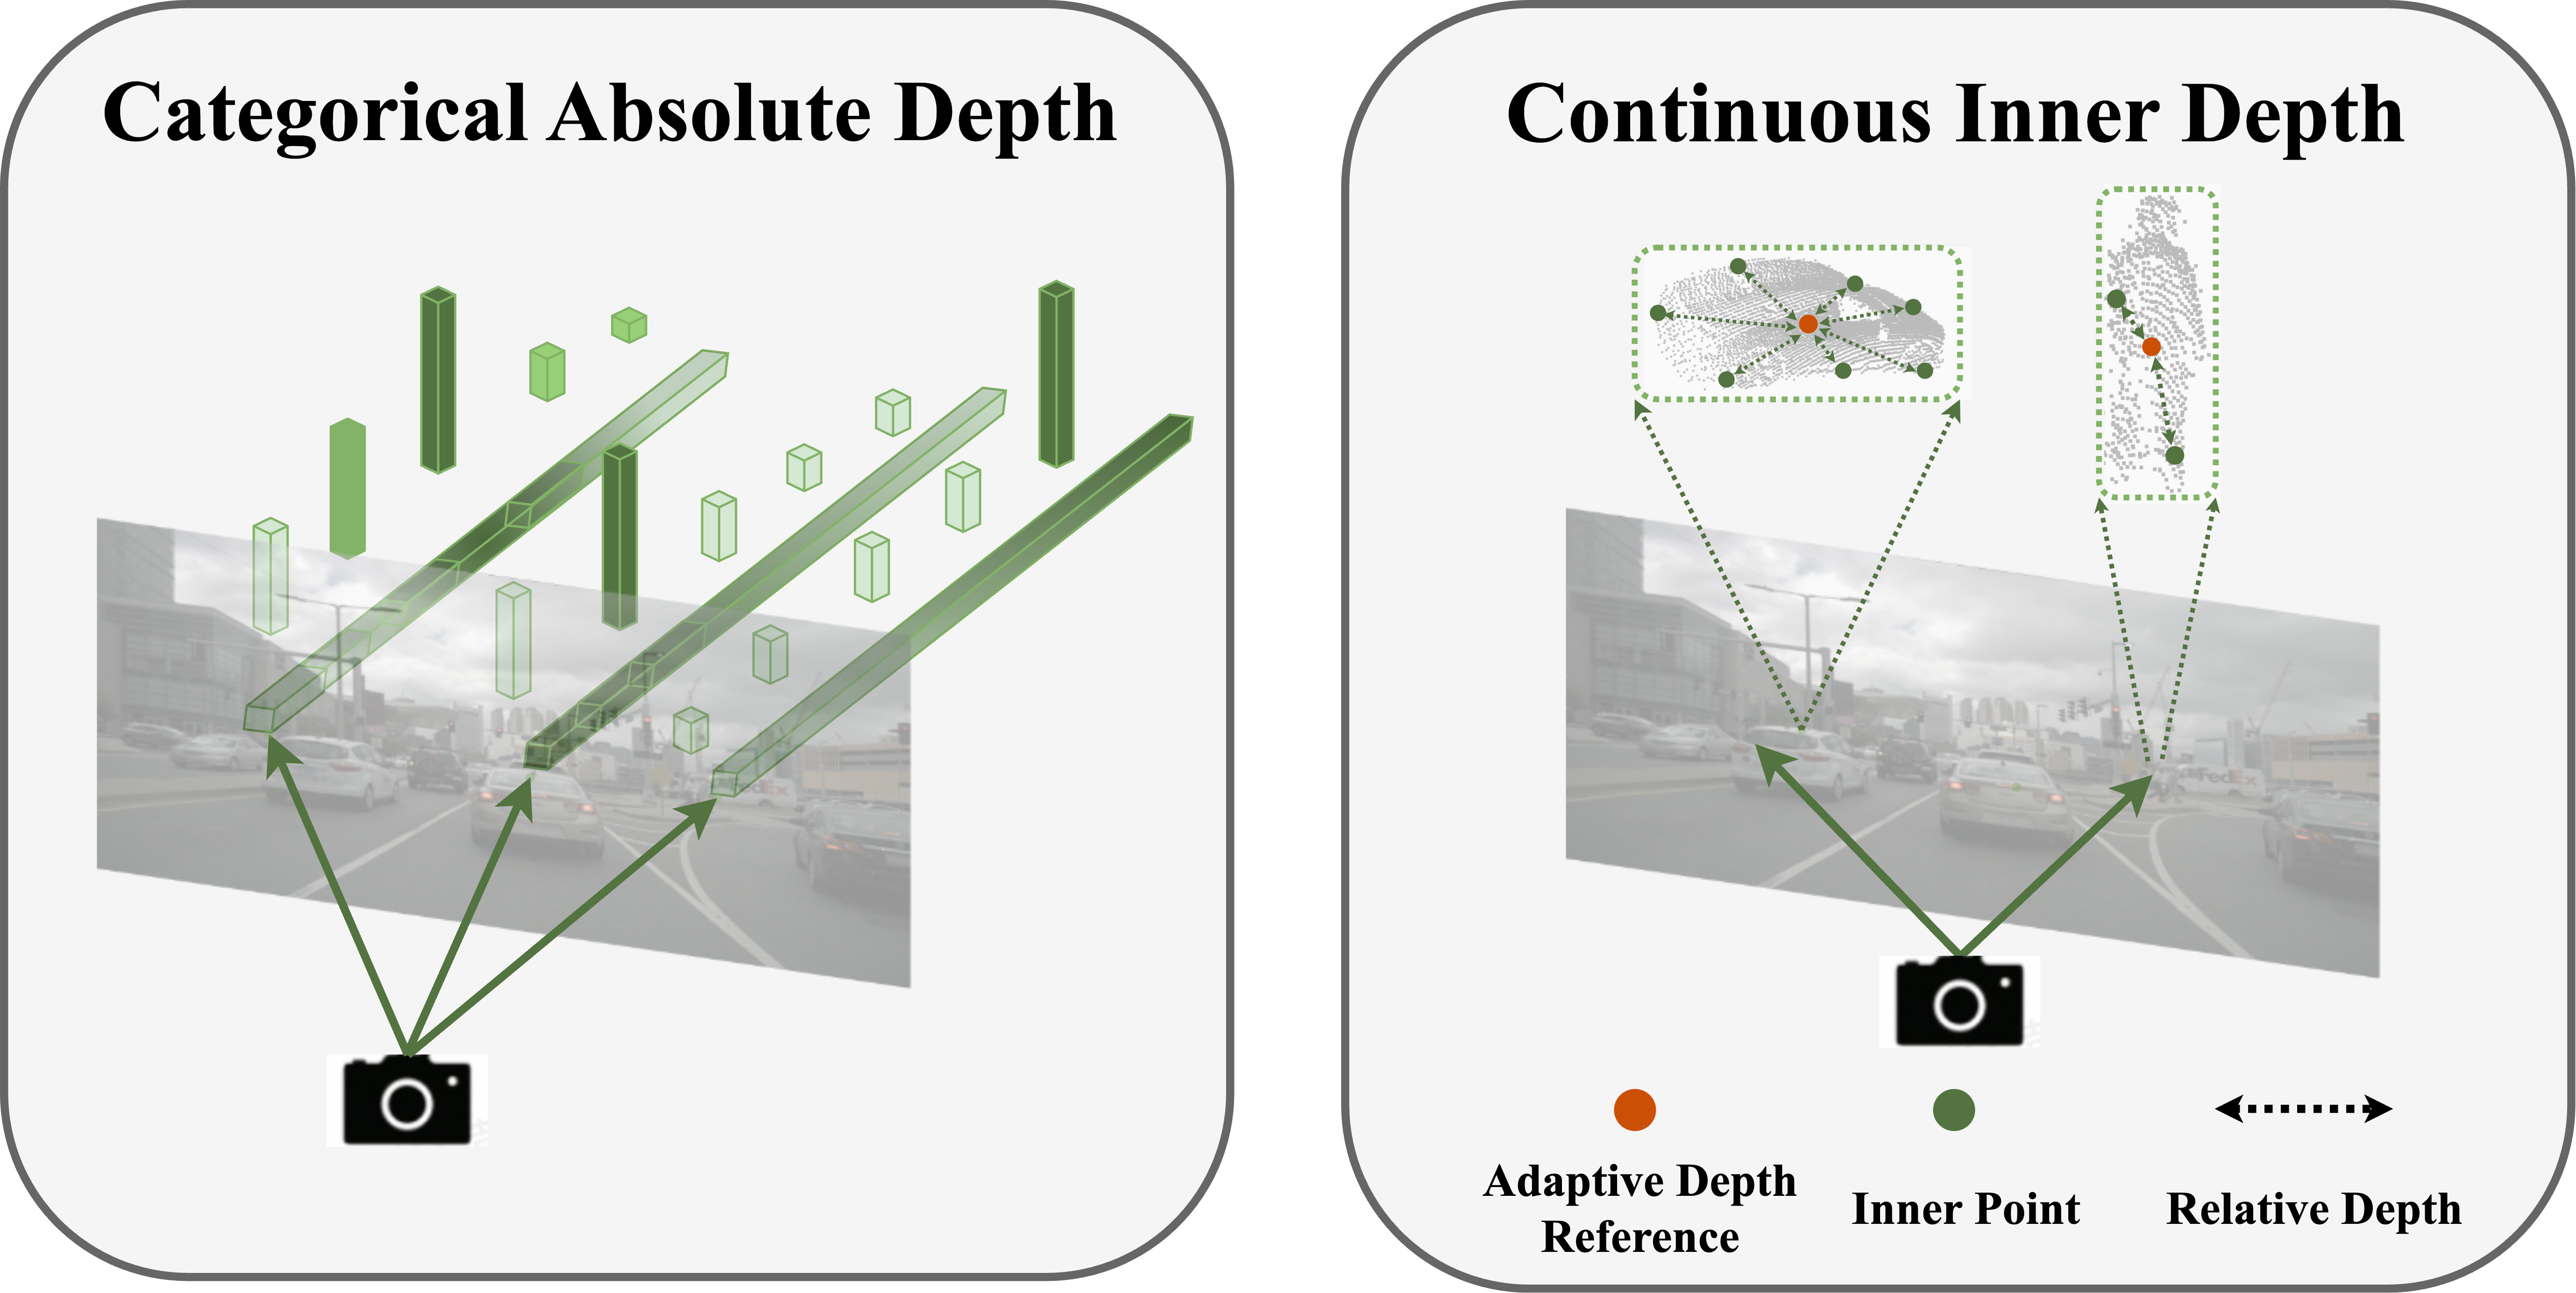
\includegraphics[scale=0.042]{cvpr_2022/iccv_fig5.drawio.png}
    \caption{\textbf{Comparison of Categorical Absolute Depth and Continuous Inner Depth.} We adopt the inner-depth supervision with continuous depth values to guide the camera-based student to learn local spatial structures of foreground object targets.
    }
    \label{fig:relative_depth}
    % \vspace{-0.8cm}
\end{figure}

%Start with $N$ ground truth 3D bounding boxes $\bm{B_{gt}}= \{\bm{b}_{i}\}_{i=1}^{N}$, which contains box center position, size and heading angle. We then obtain points in each 3D bounding boxes $\bm{P_{gt}}= \{\bm{P}^{pc}_i\}_{i=1}^{N}$, ${P}^{pc}_i$ means point clouds $P$ within 3d bounding box ${b}_{i}$. Take an object instance as example, we project ${P}^{pc}_i$ on image coordinate. 

%\begin{equation}
%    \hat{P_i^{}}(ud, vd, d) = K_{i}(R_i P_{i} + t_i),
%\end{equation}
 %In the section 3.1, we consider the depth estimation as a classification problem of the depth distribution. For the defined depth bins $b_i$, we interpret the $D$ Softmax scores, $p_k$, $k=1,..,D$, and choose the final prediction depth $b^{k}_i$ at highest prediction confidence bin. 

% In the absolute depth supervision, we apply one hot encoding to ${D_i}^{gt}$ considering the depth estimation as a classification problem of the depth distribution, first adopted in BEVDepth \cite{b7}. We divided the depth distance into D depth bins, the depth-bin-centers set denoted as ${\mathbf{B_i}=\{b^1_i, b^2_i,..., b^k_i,... b^D_i\}}$ , and we interpret the $D$ Softmax scores, $p^{k}_i$, $k=1,..,D$ at each pixel as probabilities over the ${\mathbf{B_i}}$ vector, and choose the final prediction depth $b^{k}_i$ at highest prediction confidence bin. 
%  \begin{equation}
%  \label{eq:FM}
%  \begin{aligned}
%     D_i = b^{k}_i {\max_{k=1}^D {{p^{k}_i}}}.
%  \end{aligned}
%  \end{equation}
% Here, we want to calculate the exact relative depth for different pixels within the target, the discrete depth prediction like above is not enough to express the tiny depth difference. Thus, for the further accurate prediction depth and can be used for the relative depth relation among different pixels within the certain ROI, we calculate the final depth value $\hat{D_i}$ by the hybrid mean regression as follow:
%  \begin{equation}
%  \label{eq:FM}
%  \begin{aligned}
%     {\hat{D_i}} = {\sum_{k=1}^D {{b^{k}_i}{p^{k}_i}}}.
%  \end{aligned}
%  \end{equation}
 % Compared the discrete depth prediction, we do not predict the depth as the chosen likely bin. This enables us to predict smooth depth without the discriminative artifacts, which helps to obtain the complete representation of the geometry depth.  
 
 \paragraph{Adaptive Depth Reference.}
 To calculate the relative depth values, we propose to utilize an adaptive depth reference for different foreground targets.
 Specifically, according to the predicted continuous depth values in $\{\hat{S_j}\}_{j=1}^M$, we select the pixel with the smallest depth prediction error as the reference point for each target, and correspondingly set its depth value as the depth reference, as shown in Figure~\ref{fig:relative_depth}. For the $j$-th target with the ground-truth inner-depth $\{\hat{S_j}, \hat{S^{gt}_j}\}_{j=1}^M$, we calculate the depth reference point $(x_r, y_r)$ by
  \begin{equation}
 \label{eq:FM}
 \begin{aligned}
    (x_r, y_r) = \mathop{\text{Argmin}}_{(x, y)\in \hat{S_j}} \left ({S^{gt}_j}(x, y) - {\hat{S_j}}(x, y)\right ).
 \end{aligned}
 \end{equation}
 Then, the predicted and ground-truth reference depth values are denoted as $d_j(x_r, y_r)$ and $d^{gt}_j(x_r, y_r)$, respectively. By adaptively selecting the reference point with the smallest error, the inner-depth distribution can dynamically adapt to objects with different shapes and appearances, which stabilizes the network learning for some truncated and occluded objects.

\paragraph{Inner-depth Calculation.}
On top of the reference depth value, we calculate the relative depth values within the foreground area of each target object. For pixel $(x, y)$ of the $j$-th target $\{\hat{S_j}, S_j^{gt}\}$, the predicted and ground-truth inner-depth values are formulated as
\begin{equation}
 \label{eq:FM}
 \begin{aligned}
    rd_j(x, y) &= d_j(x, y) - d_j(x_r, y_r),\\
    rd^{gt}_j(x, y) &= d^{gt}_j(x, y) - d^{gt}_j(x_r, y_r).
 \end{aligned}
 \end{equation}
 We denote the obtained relative depth-value sets for $M$ target objects as $\{\hat{R_j}, R_j^{gt}\}_{j=1}^M$. Finally, we supervise the inner-depth prediction of the student detector by an L2 loss, formulated as
 \begin{equation}
\label{eq:FM}
    \mathcal{L}_{\rm{depth}}^{R} = \sum_{j=1}^M ||\hat{R}_{j}-R^{gt}_{j}||_2.
\end{equation}
 
%  When we set the inner point and the reference point within the ROI, we can define the two relative depth sets ${\mathbf{\hat{D}}^{gt}}$ ${\mathbf{\hat{D}}^{pred}}$ of the pixels with cardinality ${M}$. 
% \begin{equation}
%     {\mathbf{\hat{D}}^{gt}} = 
% \left[{\hat{D}^{gt}_{1r},\hat{D}^{gt}_{2r},\cdots,\hat{D}^{gt}_{ir},\hat{D}^{gt}_{Mr}}\right].
% \end{equation}
% \begin{equation}
%     {\mathbf{\hat{D}}^{pred}} = 
% \left[{\hat{D}^{pred}_{1r},\hat{D}^{pred}_{2r},\cdots,\hat{D}^{pred}_{ir},\hat{D}^{pred}_{Mr}}\right].
% \end{equation}
%  where the ${\hat{D}_{ir}^{gt}}=\hat{D}_i^{gt}-\hat{D}_r^{gt}$ and ${\hat{D}_{ir}^{pred}=\hat{D}_i^{pred}-\hat{D}_r^{pred}}$ denotes the relative depth distance of the lidar pixels and cam pixels. 
 
%  To obtain the inner-geomtry depth relation from the lidar points, we minimize the discrepancy between the above sets in a one-to-one relative spatial matching manner. 
% \begin{equation}
% \label{eq:FM}
%     \mathcal{L}_{\rm{Rdepth}} = ||{\mathbf{\hat{D}}^{gt}}-{\mathbf{\hat{D}}^{pred}}||_2 = \sum_{i=1}^M ||\hat{D}^{gt}_{ir}-\hat{D}^{pred}_{ir}||_2.
% \end{equation}
%% \KY{focus on semantic mismatch}
%\noindent This formulation assumes that the semantic distributions of the teacher and the student match exactly. 
% However, a recent study~\cite{Cho2019OnTE} observes that small students are inefficient to mimic large teachers. 
%However, as mentioned earlier, for the feature maps of the teacher network, which usually encompasses more layers and larger feature channels, the spatial information of the same pixel location contains a richer semantic information compare to the student network. Directly regressing the features in a pixel-wise manner may lead to suboptimal distillation results. 
% has a stronger learning capability (\eg larger receptive field) and richer representation. That means the semantic of spatial components of teacher and student usually varies. Directly linking the teacher and student by spatial order may trigger the issues of semantic mismatch and lead to sub-optimal results.
% \KY{this is not helping the story, size difference is one reason that KD is hard. but our approach does not help in this way} 
% As the teacher grows in capacity and accuracy, the student often finds it difficult to emulate the teacher. 
% To this end, we propose to guide the whole student to mimic each spatial component of the teacher respectively. In this way, we can increase the matching capability and subsequently improve the knowledge distillation performance.

%This formulation does not consider the gap of expressivity and the exact semantic distance between $f^s_i$ and $f^t_i$, which may introduce bias. To address the limitation of Eq. \ref{eq:FM}, we reconfigure each elements in set $f^s$ by a target-aware transformer. 
%A straightforward solution is to measure the semantic distance between the elements of two sets and then assign the $f^t_i$ with the most semantic-related one from $f^s$. As we will demonstrate, this is the special case of our proposed method.
%To this end, we propose a one-to-all spatial matching knowledge distillation pipeline that allows the each feature location of the teacher to teach the entire student features in a dynamic manner.
%To make the whole student mimic a spatial component of the teacher, we propose the \textbf{T}arget-\textbf{a}ware \textbf{T}ransformer (\textbf{TaT}) to pixel-wisely reconfigure the semantic of student feature in the certain position.
%We propose the Target-aware Transformer (\textbf{TaT}) to pixel-wisely reconfigure the semantic of student feature in the certain position. 
%Given a spatial component (alignment target) of the teacher, we use \textbf{TaT} to guide the whole student to reconstruct the feature in its corresponding location. Conditioned on the alignment target,  \textbf{TaT} should reflect the semantic similarity with the components of the student feature. We use a linear operator to avoid changing the distribution of student semantics. The formulation of transformation operator $W^i$ can be defined as:
%Given the alignment target $f^t_i$, \textbf{TaT} is to find the weights $W^i$ that controls the flow of semantic aggregation across the student feature w.r.t the $i$-th pixel of student feature. Conditioned on the alignment target, \textbf{TaT} should reflect the semantic similarity with the components of the student feature. Also, it should be a linear operator otherwise it changes the distribution of student semantics. The formulation of $W^i$ can be defined as:
%\begin{equation}
%\label{eq:spe}
%\begin{aligned}
%   W^i&= \sigma(\langle {f^s_1},{f^t_i}\rangle,\langle {f^s_2},{f^t_i}\rangle,\dots,\langle {f^s_N},{f^t_i}\rangle)\\
%   &=[{w^i_1},{w^i_2},\dots,{w^i_N}],
%\end{aligned}
%\end{equation}
%\noindent where $f^t_i$ and $f^s_i$ denote the corresponding $i$-th components of teacher and student, $\langle \cdot,\cdot \rangle$ represents the inner-product and  $\|W^{i}\|=1$. We use inner-product to measure the semantic distance and softmax function for normalization. 
%Note that if we only reserve the entry of the maximum of $W^{'}$, it degrades to the nearest-neighbor. 
% Here $W^{i}$ is the gate that guides the semantic flow to the reconfigured point ${f^s_i}^{'}$. 



%Note this is the simple non-parametric method that only depends on the original features. To facilitate the training, we introduce the parametric method with the extra linear transformation applied on the student feature and teacher feature. We observe that parametric version performs better than non-parametric one in ablation study. Guided by the target-aware transformer, the reconfigured student feature can be formulated as: 
% \KY{why we need parameteric formulation? does non-param work? do we have the experiment? if not, consider to do this in supplementary}
% Also, the issue of semantic mismatching may occur in the channel dimension. To address this issue, we propose to partition the feature tensor along the channel dimension and performs the self-assembling in parallel:
%\begin{equation}
%\label{eq:mul-self-essem}
%    {f^s}^{'}=\sigma(\gamma(f^{s})\cdot \theta({f^t})^{\top})\cdot \phi(f^{s}),
%\end{equation}
%\noindent where $\theta(\cdot)$, $\gamma(\cdot)$ and $\phi(\cdot)$ are the linear functions consisting of $3\times 3$ conv layer plus the BN layer \cite{ioffe2015batch}. We compare the parametric \textbf{TaT} to non-parametric one to analyse the effectiveness brought by these linear functions in the Section~\ref{sec:ablation}. 
%In the case that the channel numbers of $F^S$ do not match with that of $F^T$, $\gamma(\cdot)$ can help with alignment.

% \KY{where? point the section} 
%The resulting \textbf{TaT} map ($\gamma(f^{s})\cdot \theta({f^t})^{\top}$) is of size $\mathbb{R}^{HW \times HW}$, which is acceptable considering that most classification networks have small feature map size on the top layers. On ResNet18, the spatial size of feature map in the 4-th block is, for example, $7\times7$.  \KY{discuss the complexity in the next section...}

%After reconfiguration, each component of ${f^s}^{'}$ aggregates the meaningful semantic from the original feature, which enhances the expressivity. We do not require the student to reconstruct the teacher feature in a pixel-to-pixel manner. Indeed, our model allows the student to act as a whole to mimic the teacher. The resulting ${f^s}^{'}$ is lately asked to minimize the L$_2$ loss with the teacher feature. The objective for \textbf{TaT} knowledge distillation can be given by:
%\begin{equation}
%    \mathcal{L}_{\rm{TaT}}= ||{f^s}^{'}-f^t||_2.
%    \label{eq:fm}
%\end{equation}

% \KY{this only apply to Cls? how about other loss? consider change cls $\rightarrow$ task. L_T -> $L_{TaT}$ }
%Finally, the total loss of our proposed method can be defined by: 

%\begin{equation}
%\label{eq:objective}
    %\mathcal{L}=\alpha\mathcal{L}_{\rm{Task}}+\beta\mathcal{L}_{\rm{KL}}+\epsilon\mathcal{L}_{\rm{TaT}},
%\end{equation}
%\noindent Here $\mathcal{L}_{\rm{Task}}$ can be any loss on the generic machine learning tasks. $\alpha$, $\beta$ and $\epsilon$ are the weight factors to balance the loss. 
%Empirically, we find that our model benefits from $\mathcal{L}_{\rm{KL}}$. However, the model can achieve state-of-the-art without the help of $\mathcal{L}_{\rm{KL}}$.
% , \ie, $\beta$ is set to 0. \KY{this is strange... why mentioning this if we set beta = 0??}

% \subsection{Empirical \& Theoretical Analysis}
% This section provides some intuition to the formulation discussed above. Without loss of generality, let's remove the linear functions $\theta(\cdot)$ and $\gamma(\cdot)$ and consider only one attention head. The Eq. \ref{eq:fm} can be expressed in another way:
% \begin{equation}
%     softmax(X\cdot Y^{\top})\cdot X=Y.
% \end{equation}
% \noindent Here $softmax(X\cdot Y)$ is the cross-attention matrix which is applied to the student feature $X$. The objective for the student is to reconstruct the teahcer feature. Denote the optimum solution to $X$ as $\hat{X}$. The non-trivial solution indeed requires that $softmax(\hat{X}\cdot Y^{\top})=I$ and $\hat{X}=Y$.

% Recall that each raw of $X$ and $Y$ corresponds to a pixel in the original feature tensor. By means of matrix multiplication, it calculates the inner-product of each paired pixels between student and teacher, resulting the cross-attention matrix. The inner-product between two pixels measures the similarity against difference, and it's normalized by the softmax function. Since the cross-attention matrix is required to be the identity matrix, this can be interpreted that the distance, reflected by the inner-product, of the associated positions between $f_s$ and $f_t$ should be as close as possible, otherwise distant. This is the necessary condition if $\hat{X}=Y$ holds.

% We now begin to give a theoretical analyse to the existence of the solution $\hat{X}$. Because student feature is expected to match the teacher feature, we have $\hat{X}=Y$. Thus, we need to prove that $softmax(Y,Y^{\top})=I$. We presume that the elements of $Y$ is Gaussian distribution and each raw is not linearly dependent from each other. Here $Y$ can be represented as:
% \begin{equation}
% \begin{aligned}
%   Y=[{y_1}^{\top},{y_2}^{\top},{y_3}^{\top},\dots,{y_N}^{\top}]^{\top},\\
% \end{aligned}
% \end{equation}
% \noindent where $Y$ has $N=H\cdot W$ raw vectors. Suppose that $y_i$ and $y_j$ are two distinct vectors, they can be described as:
% \begin{equation}
% \begin{aligned}
%   y_i=[y_{i,1},y_{i,2},y_{i,3},\dots,y_{i,C}],\\
%   y_j=[y_{j,1},y_{j,2},y_{j,3},\dots,y_{j,C}],\\
% \end{aligned}
% \end{equation}
% where $(1\leq i,j\leq N)$ and each vector is of length $C$. The expected value of the inner-product of two vectors can be given by:
% \begin{equation}
% \label{eq:in_prd_same}
%     \begin{aligned}
%       \mathbb{E}\langle y_i,y_i\rangle &= \mathbb{E}(y_{i,1}^2+y_{i,2}^2+y_{i,3}^2+\dots+y_{i,C}^2) \\
%       &=\sum_{k=1}^{C}\mathbb{E}y_{i,k}^2= \sum_{k=1}^{C}(\mu_{i,k}^2+\sigma_{i,k}^2)=C ,
%     \end{aligned}
% \end{equation}

% \begin{equation}
% \label{eq:in_prd_diff}
%     \begin{aligned}
%       \mathbb{E}\langle y_i,y_j\rangle 
%       &= \mathbb{E}(y_{i,1}\cdot y_{j,1}+y_{i,2}\cdot y_{j,2}+\dots+y_{i,C}\cdot y_{j,C}) \\
%       &=\sum_{k=1}^{C}\mathbb{E}(y_{i,k}\cdot y_{j,k})\\
%       &=\sum_{k=1}^C \left[ \mathbb{E}y_{i,k}\cdot \mathbb{E}y_{j,k}+Cov(y_{i,k},y_{j,k}) \right]  \\
%       &\leq \sum_{k=1}^{C}(\mu_{i,k}\cdot \mu_{j,k}+|\sigma_{i,k}\cdot \sigma_{j,k}|)\\
%       &=\rho \cdot C .
%     \end{aligned}
% \end{equation}
% Here $\mu=0$ and $\sigma=1$ is the mean and standard deviation of Gaussian distribution. The Eq. \ref{eq:in_prd_same} indicates the expected value of the inner-product between a vector and itself, while Eq. \ref{eq:in_prd_diff} illustrates the inner-product of two distinct vectors, which is derived by Cauchy–Schwarz inequality a.k.a covariance inequality. Here $0\leq \rho \leq 1$ and it equals to 1 if and only if two vectors are linearly dependent. Since we presume that vectors are not linearly dependent in matrix $Y$, we have $\rho<1$.

% Given Eq. \ref{eq:in_prd_same} and Eq. \ref{eq:in_prd_diff}, we consider the diagonal of the cross-attention matrix. Normalized with softmax function, the limiting condition of the $i$-th position of the $i$-th raw can be described by:
% \begin{equation}
% \label{eq:lim}
%     \lim_{C\to \infty} \frac{e^C}{(N-1)\cdot e^{\rho\cdot C}+e^C}=1.
% \end{equation}

% The limiting condition presented in Eq. \ref{eq:lim} means the $i$-th raw of the cross-attention map is the one-hot vector where $i$-th position is 1 as long as the feature channel is deep enough. Thus the resulting cross-attention matrix is an identity matrix. In our experiment setting, the feature tensor of 4-th layer in ResNet18 is of size $7\times 7 \times 512$, \ie $N=49$ and $C=512$. Even though $\rho$ reaches 0.98, Eq. \ref{eq:lim} can return 0.998 that is very close to 1.  

%--------------------------------------------------------------------------------

%--------------------------------------------------------------------------------
\subsection{Inner-feature BEV Distillation}
\label{sec:Inner-feature BEV Distillation}
%In this section we introduce the adaption of the model discussed previously and show its application on semantic segmentation. 
% \KY{inductive bias? do we really want to talk about this?}
% \ky{Although our one-to-all distillation approach can address the semantic mismatch, it has one limitation about the computational complexity. As the resulting correlation mapping }
% The proposed \textbf{TaT} lift the limitation of previous one-to-one spatial matching fashion. 
%For example, features in the neighborhood are more relevant to themselves, on the contrary, features that are farther away are less relevant. The student must figure out all of these in the learning process, which may be very challenging when the feature map is large.

Besides the depth supervision for low-level spatial information, our TiG-BEV also adopts the inner-geometry learning for high-level BEV semantics from pre-trained LiDAR-based detectors. 
Previous works~\cite{b9,b52} for BEV distillation directly force the student to imitate the teacher's features point-to-point in the BEV space. In spite of the performance improvement, such strategies are constrained by the following two aspects. On the one hand, due to the sparsity of scanned point clouds, the LiDAR-based BEV features might contain redundant and noisy information in the background areas. Although BEVDistill~\cite{b9} utilizes foreground masks to alleviate this issue, such dense feature distillation still cannot provide focused and effective guidance to the student network. On the other hand, the camera-based and LiDAR-based BEV features depict different characteristics of the scene, respectively, visual appearances and spatial structures. Therefore, forcing the BEV features to be completely consistent between two modalities is sub-optimal considering the semantic gap. In our TiG-BEV, we propose an inner-feature BEV distillation (Figure~\ref{fig:structure_attn}) consisting of inter-channel and inter-keypoint learning schemes, which conducts attentive target features distillation and relieve the cross-modal semantic gap.

% There are two main observations, on the one hand, the feature distribution of point clouds and images are not consistent due to the sparsity of point clouds, directly distilling on all region of features is not reasonable. On the other hand, even features of two modalities can hold meaningful information in the region of foreground, the representation of the features from different modalities are diverse in channel and spatial wise. Forcing students to imitate the foreground feature of the teacher is sub-optimal. Therefore, we propose a foreground structured attention feature supervision module to transfer more reliable relative spatial feature relationships from LiDAR-based teacher to multi-view based student. It contains of two distillation modules: 1) Inner Target-Aware distillation, 2) Local Target-Aware distillation,which..


\paragraph{Target Keypoint Extraction.}
To distill the knowledge of LiDAR-based detectors only within sparse foreground regions, we extract the BEV area of each object target and represent it by a series of keypoint features.
Given the ground-truth 3D bounding box for each target, we first enlarge the box size for a little bit in the BEV space to cover the entire foreground area, e.g., object contours and edges. Then, we uniformly sample its BEV bounding box by $N$ keypoints, and adopt bilinear interpolation to obtain the keypoint features from the encoded BEV representations. From both camera-based $F^{2d}_{\rm bev}$ and LiDAR-based $F^{3d}_{\rm bev}$, we respectively extract the keypoint features for all $M$ object targets as $\{f_j^{2d}, f_j^{3d}\}_{j=1}^M$, where $f_j^{2d}, f_j^{3d} \in {\mathbb{R}^{N\times C}}$. By the uniform sampling, such BEV keypoints can well represent the part-wise features and the inner-geometry semantics of foreground targets.

\begin{figure}[!t]
% \vspace{-0.5cm}
    \centering
    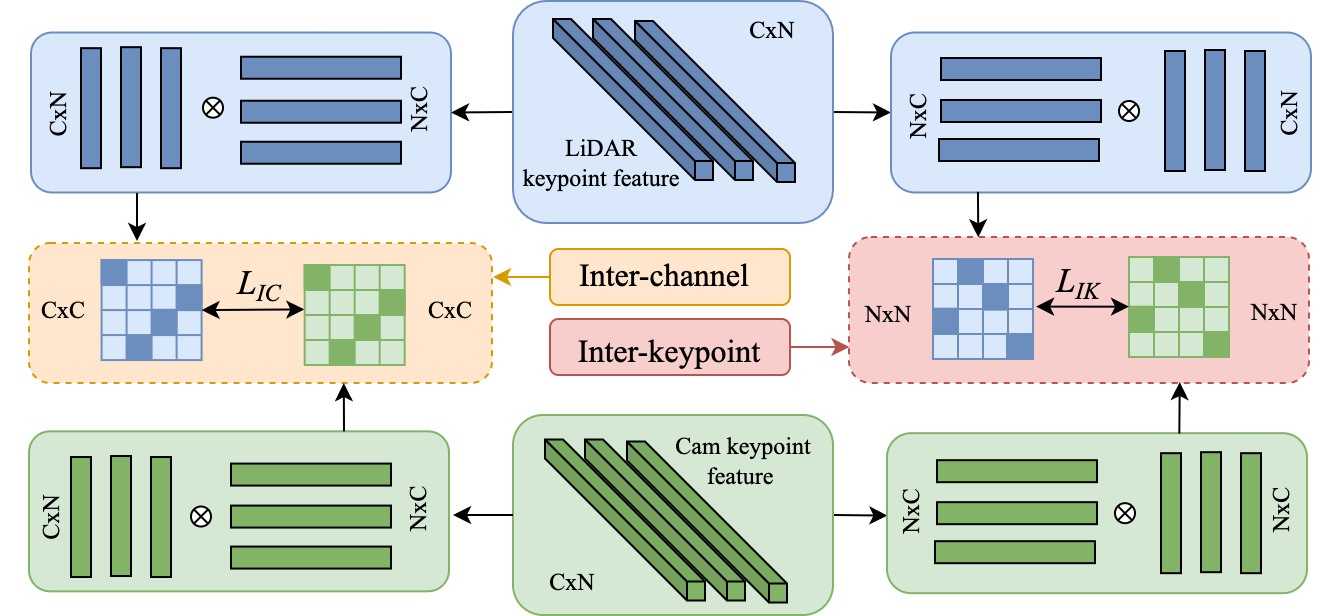
\includegraphics[scale=0.17]{cvpr_2022/iccv_fig6_2.drawio.png}
    \caption{\textbf{Detials of Innter-feature BEV Distillation.} For each foreground area in BEV space, we represent rach target feature by a set of keypoints and conduct feature distillation in both inter-channel and inter-keypoint manners.
    }
    \label{fig:structure_attn}
    % \vspace{-0.8cm}
\end{figure}

% and the corresponding background regions and divide into small grids with spatial resolution of $G_i\times G_i \times G_i$, which can summarize each foreground area into the certain number of feature keypoints.  For the bird-view feature maps, we project the keypoint $p_i$ to the 2D bird-view coordinate system and utilize bilinear interpolation to obtain the features $f^{bev}_i$ from the bird-view feature maps. Hence, the roi feature can be represented as follow:

% \begin{equation}
%     {F_i^{ROI}} = {f^{bev}_1,...,f^{bev}_i,f^{bev}_n}, 
%  i=1,..N
% \end{equation}
% which have the strong capability of preserving 3D geometry information of the foreground scene and can also boost the marginal awareness performance of the certain target.

\paragraph{Inter-channel BEV Distillation.}
% \label{sec:seq}
Taking the $j$-th object target as an example, we first apply an inter-channel BEV distillation, which guides the student keypoint features to mimic the channel-wise relationships of the teacher's. Such inter-channel signals imply the overall geometric semantics of each object target. Compared with the previous channel-by-channel supervision, our inter-channel distillation can preserve the distinctive aspects of the two modalities, while effectively transfer the well pre-trained knowledge of LiDAR-based detectors. Specifically, we calculate the inter-channel similarities of both camera-based and LiDAR-based keypoint features, formulated as
\begin{equation}
    A_j^{2d} = f_j^{2d} {f_j^{2d}}^{\top};\ \ \ A_j^{3d} = f_j^{3d} {f_j^{3d}}^{\top},
\end{equation}
where $A_j^{2d}, A_j^{3d} \in {\mathbb{R}^{C\times C}}$ denote the feature relationships between different $C$ channels for the two modalities. For all $M$ objects in a scene, we adopt L2 loss between the two inter-channel similarities for feature distillation, formulated as
\begin{equation}
    \mathcal{L}_{\rm{bev}}^{{IC}}= \sum_{j=1}^{M} ||A_j^{3d}-A_j^{2d}||_2.
    \label{eq:fm}
\end{equation}

% Given the RoI feature of each box proposal, the lidar-based bev feature and cam-based bev feature can be represented as $F_i^{Lidar}\in {\mathbb{R}^{N\times C}}$, $F_i^{cam}\in {\mathbb{R}^{N\times C}}$ respectively, where ${N}$ represents the number of keypoints and ${C}$ represents the channels numbers. For the certain sampled feature of the keypoint, it reflects the certain information within the receptive field. As mentioned before, the lidar-based detector has the better detection performance since the spatial information of the same inner roi location contains the richer semantic information compare to the cam-based detector. Thus, we propose a inner target-aware (\textbf{ITA}) distillation that performs distillation within channel wise, which allows student to learn the context of feature from RoI patches and retain the correlation among different channels. For the bev feature ${i}$th ROI, the channel-wise information matrix is defined as: 
% \begin{equation}
%     {G_i^{ROI}} = {F^{Lidar}_i\cdot {F^{Lidar}_i}}^{\top}
% \end{equation}
% The information matrix has a size of ${C\times C}$ regardless of the spatial dimension ${N}$. ${G_{i,(m,n)}^{ROI}}$ denotes the inner channel correlation between $m$th channel and $n$th channel for the same location of the $i$th ROI.

% \begin{equation}
% \begin{aligned}
% %L_{task} = &\lambda_1 L_{per}(G_s(x),G_t(x))  +\lambda_1  L_{CE}(y,\delta(z_s))\\ & + \lambda_1L_{Focal}(y,y_{out})
% %{G_{i,(m,n)}^{ROI}} = &{f^_{1,m}}{f^_{1,n}}^{\top}  +{f^_{2,m}}{f^_{2,n}}^{\top} + \dots + \\&{f^_{N,m}}\cdot {f^_{N,n}}^{\top}
% {G_{i,(m,n)}^{ROI}} = &{f^_{1,m}}\cdot {f^_{1,n}}^{\top} + {f^_{2,m}}\cdot {f^_{2,n}}^{\top}\\ & + \dots + \\{f^_{N,m}}\cdot {f^_{N,n}}^{\top}
% \end{aligned}
% \end{equation}


% For the same roi area, to make the whole cam-based detector mimic
% a spatial component of the lidar-based detector, we use the Inner-target aware operator ${G_{i,(m,n)}^{ROI}}$ to pixel-wisely reconfigure the
% semantic of cam-based feature in the certain position and transfer the channel correlation of the lidar-based feature to the cam-based feature in the certain position. Conditioned on the same roi, the ${G_{i,(m,n)}^{ROI}}$ should reflect the semantic similarity with between the components. 

% We penalize the $L_2$ distance between the channel-wise information matrix of the lidar-based detector and the cam-based detector, allowing the cam-based to obtain the similar feature diversity for the same foreground area.
% \begin{equation}
%     \mathcal{L}_{\rm{ITA}}= ||G^{Lidar}_{i,cha}-G^{cam}_{i,cha}||_2.
%     \label{eq:fm}
% \end{equation}


\begin{table*}[ht]
\centering
\caption{\textbf{Performance Comparison on nuScenes~\cite{b6} Val Set.} 'C' and 'L' denote the camera-based and LiDAR-based methods, which refer to the input data during inference. * denotes our implementation using BEVDet\cite{b19} codebase.
%using their official codes.
% We have at least 1 absolute point of performance gain against KD \cite{Hinton2015DistillingTK} on 5 out of 7 experimental settings.
}
%\vspace{-0.2cm}
\resizebox{2\columnwidth}{!}{
\tablestyle{5pt}{1.2}
\begin{tabular}{c|c|c|c|cc|ccccc}
\toprule[1.2pt]
Method          & Modality & Backbone & Resolution & mAP↑  &NDS↑& mATE↓ & mASE↓ & mAOE↓ & mAVE↓ & mAAE↓   \\ \midrule
FCOS3D\cite{b12}          & C  &ResNet-101 & 900 $\times$ 1600 & 0.343& 0.415 & 0.725 & 0.263 & 0.422 & 1.292 & 0.153  \\
PGD\cite{b17}             & C  &ResNet-101 & 900 $\times$ 1600 & 0.369& 0.428 & 0.683 & 0.260 & 0.439 & 1.268 & 0.185  \\
MonoDETR\cite{b47}             & C  &ResNet-101 & 900 $\times$ 1600 & 0.372& 0.434 & 0.676 & 0.258 & 0.429 & 1.253 & 0.176  \\
%BEVDepth-R50        & C &ResNet-50   & 256 \times 704  & 0.351 & 0.639 & 0.267 & 0.479 & 0.428 & 0.198 & 0.475 \\
% BEVDepth\cite{b7}         & C &ResNet-101  & 512 \times 1408 & 0.412 & 0.565 & 0.266 & 0.358 & 0.331 & 0.190 & 0.535 \\
DETR3D\cite{b13}          & C &ResNet-101  & 900 $\times$ 1600 & 0.303& 0.374 & 0.860 & 0.278 & 0.437 & 0.967 & 0.235  \\
PETR\cite{b21}            & C  &ResNet-101    & 512 $\times$ 1408 & 0.357 & 0.421& 0.710 & 0.270 & 0.490 & 0.885 & 0.224  \\
BEVFormer\cite{b11}       & C  &ResNet-101   & 900 $\times$ 1600 & 0.416 & 0.517& 0.673 & 0.274 & 0.372 & 0.394 & 0.198   \\
PETRv2\cite{b24}            & C  &ResNet-101    & 640 $\times$ 1600 & 0.421& 0.524 & 0.681 & 0.267 & 0.357 & 0.377 & 0.186  \\
MonoDETR-MV\cite{b48}            & C  &ResNet-101    & 640 $\times$ 1600 & 0.428 & 0.531 & 0.676 & 0.268 & 0.352 & 0.380 & 0.169  \\ \midrule
CenterPoint~\cite{b53} (Teacher)   & L &VoxelNet   & -          & 0.564 & 0.646& 0.299 & 0.254 & 0.330 & 0.286 & 0.191  \\ \midrule
BEVDet$^*$ \cite{b19} & C &ResNet-50   & 256 $\times$ 704 & 0.298& 0.379 & 0.725 & 0.279 & 0.589 & 0.860 & 0.245  \\ 
\rowcolor{gray!12} \textbf{+ TiG-BEV}     &C  &ResNet-50  & 256 $\times$ 704 & \textbf{0.331} & \textbf{0.411}& 0.678 & 0.271 & 0.589 & 0.784 & 0.218  \\ 
\rowcolor{gray!12}& &&& \textbf{\textcolor{blue}{+3.3$\%$} }& \textbf{\textcolor{blue}{+3.2$\%$}}&\textcolor{blue}{-4.7$\%$} & \textcolor{blue}{-0.8$\%$} & \textcolor{blue}{-0.0$\%$} & \textcolor{blue}{-7.6$\%$} & \textcolor{blue}{-2.7$\%$}   \\ 
\midrule
BEVDet4D$^*$ \cite{b23} & C &ResNet-50   & 256 $\times$ 704 & 0.322 & 0.451& 0.724& 0.277& 0.520 &0.366 &0.212  \\
\rowcolor{gray!12} \textbf{+ TiG-BEV}     & C &ResNet-50  & 256 $\times$ 704 & \textbf{0.356}& \textbf{0.477} & 0.648 & 0.273 & 0.517 & 0.364 & 0.210  \\ 
\rowcolor{gray!12}& &&& \textbf{\textcolor{blue}{+3.4$\%$} }& \textbf{\textcolor{blue}{+2.6$\%$}}&\textcolor{blue}{-7.6$\%$} & \textcolor{blue}{-0.4$\%$} & \textcolor{blue}{-0.3$\%$} & \textcolor{blue}{-0.2$\%$} & \textcolor{blue}{-0.2$\%$}   \\ 
\midrule
BEVDepth$^*$ \cite{b7} & C &ResNet-101   & 512 $\times$ 1408 & 0.416 & 0.521& 0.605 & 0.268 & 0.455 & 0.333 & 0.203  \\
\rowcolor{gray!12}   \textbf{+ TiG-BEV}   & C & ResNet-101  & 512 $\times$ 1408  & \textbf{0.440}& \textbf{0.544} & 0.570 & 0.267 & 0.392 & 0.331 & 0.201  \\ 
\rowcolor{gray!12}& &&& \textbf{\textcolor{blue}{+2.4$\%$} }& \textbf{\textcolor{blue}{+2.3$\%$}}&\textcolor{blue}{-3.5$\%$} & \textcolor{blue}{-0.1$\%$} & \textcolor{blue}{-6.3$\%$} & \textcolor{blue}{-0.2$\%$} & \textcolor{blue}{-0.2$\%$}   \\ 
\bottomrule[1.2pt]
\end{tabular}
}

\label{tab:nus_val_sota}
%\vspace{-3mm}
\end{table*}
\paragraph{Inter-keypoint BEV Distillation.}
\label{sec:anchor}
The inter-channel distillation guides the camera-based detector to learn the channel-wise diversity from the LiDAR-based teacher. However, it is conducted without considering the inner correlation of different keypoints within each object target, which is not capable of capturing the local geometries among different foreground parts, e.g., the front and rear of cars. To this end, we propose to utilize the inter-keypoint correlations of LiDAR-based BEV features and transfer such inner-geometry semantics into camera-based detectors. Analogous to the aforementioned inter-channel module, for the $j$-th target object, we calculate the inter-keypoint similarities in a transposed manner for the two modalities as
\begin{equation}
    B_j^{2d} = {f_j^{2d}}^{\top} {f_j^{2d}};\ \ \ B_j^{3d} = {f_j^{3d}}^{\top} {f_j^{3d}},
\end{equation}
where $B_j^{2d}, B_j^{3d} \in {\mathbb{R}^{N\times N}}$ denote the feature relationships between different $N$ keypoints respectively for camera and LiDAR. We also adopt L2 loss for all $M$ targets as
\begin{equation}
    \mathcal{L}_{\rm{bev}}^{{IK}}= \sum_{j=1}^{M} ||B_j^{3d}-B_j^{2d}||_2.
    \label{eq:fm}
\end{equation}
Then, the distillation loss for inter-channel and inter-keypoint features in BEV space is formulated as
\begin{equation}
    \mathcal{L}_{\rm{bev}}=
    \mathcal{L}_{\rm{bev}}^{{IC}}+
    \mathcal{L}_{\rm{bev}}^{{IK}},
    \label{eq:seg}
\end{equation}
where the two terms are orthogonal respectively for the channel-wise feature diversity and keypoint-wise semantic correlations.

% The attempt to preserve the local correlation through concatenating all the position would fail. 
% We hope that detector can capture the context from the one position to another within the target area. In this case, the cam-based detector will, however, be distracted from the locality since the \textbf{ITA} encodes all the related semantic over the whole feature among different positions. In other words, the \textbf{ITA} will aggregates redundant local semantic.
% Furthermore, a large feature map will hinder the inductive bias since it may encourage the student to integrate the less relevant semantic from remote positions by mistake, which may deteriorate the subsequent distillation performance.
% For complex scenes and similar targets, the postion wise dependency is important to capture the relation (\eg layout) of different components within the target.

% We address the conundrum by the proposed local target-aware(\textbf{LTA}) distillation. Like the the channel-wise information matrix defined in \textbf{ITA}, the position-wise matrix is defined as follow:
% \begin{equation}
%     {G_{i}^{pos}} = {{F^{Lidar}_i}^{\top}\cdot F^{Lidar}_i}
% \end{equation}

% The information matrix has the size of ${N\times N}$ regardless of the channel dimension ${C}$. ${G_{i,(p,q)}^{pos}}$ denotes the inner spatial correlation between $p$th keypoint and $q$th keypoint for the $i$th ROI. Similarly, the formulation of the operator can be defined as:

% \begin{equation}
% \begin{aligned}
%     {G_{i,(p,q)}^{pos}} = {f^_{p,1}}\cdot {f^_{q,1}}^{\top} + {f^_{p,2}}\cdot {f^_{q,2}}^{\top} + \dots + \\{f^_{p,C}}\cdot {f^_{q,C}}^{\top}
% \end{aligned}
% \end{equation}

% After reconfiguration, the spatial relationship within the target can be extracted and summerized, which is complementary to the channel relationship. Therefore, as the cam-based detector, we enhance its gemetry expressivity by asking them to mimic the teacher. Thus, the objective for (\textbf{LTA}) knowledge distillation can be given by:

% \begin{equation}
%     \mathcal{L}_{\rm{LTA}}= ||G^{Lidar}_{i, pos}-G^{Cam}_{i, pos}||_2.
%     \label{eq:fm}
% \end{equation}

\subsection{Overall Loss}
\label{sec:overall_loss}
To sum up, we benefit the student camera-based detector by target inner-geometry from two complementary aspects, i.e., an inner-depth supervision for low-level signals and an inner-feature BEV distillation for high-level semantics. They produce two losses as $\mathcal{L}^R_{\rm{depth}}$ and $\mathcal{L}_{\rm{bev}}$. Together with the original two losses, i.e., dense absolute depth supervision $\mathcal{L}^A_{\rm{depth}}$, and 3D detection $\mathcal{L}_{\rm{det}}$, the overall loss of our TiG-BEV is formulated as
\begin{equation}
    \mathcal{L}_{\rm{TiG}}=
    \mathcal{L}_{\rm{det}}+
    \mathcal{L}^A_{\rm{depth}}+
    \mathcal{L}^R_{\rm{depth}}+
    \mathcal{L}^{IC}_{\rm{bev}}+
    \mathcal{L}^{IK}_{\rm{bev}}.
    \label{eq:seg}
\end{equation}

% The inner target-aware distillation enables the detector to mimic the inner feature diversity while the local target-aware distillation allows it to learn the local representation over the spatial feature, which are complementary to each other. Therefore, the combination of these two objectives can bring the best of two worlds. Our objective designed for structured attention feature supervision can be written by:
% \begin{equation}
%     \mathcal{L}_{\rm{SAF}}=
%     \delta\mathcal{L}_{\rm{ITA}}+
%     \zeta\mathcal{L}_{\rm{LTA}}
%     \label{eq:seg}
% \end{equation}



% Finally, the total loss of our proposed method can be defined by:
% \begin{equation}
%     \mathcal{L}_{\rm{TiG}}=
%     \mathcal{L}_{\rm{det}}+
%     \mathcal{L}^A_{\rm{depth}}+
%     \mathcal{L}^R_{\rm{depth}}+
%     \mathcal{L}^{IC}_{\rm{bev}}+
%     \mathcal{L}^{IK}_{\rm{bev}}
%     \label{eq:seg}
% \end{equation}
% Here $L_{task}$ is the loss of the 3D detection task. $\alpha$, $\beta$, $\gamma$, $\delta$ and $\zeta$ are the weight factors to balance the loss.


%-------------------------------------------------------------------------
\vspace{0.2cm}
\section{Experiment}
\label{sec:experiment}
In this section, we first introduce our adopted dataset and implementation settings. Then, we conduct a series of experiments with detailed ablation studies to show the effectiveness of our approach.

\subsection{Experimental Settings}
% \KY{which dataset do we use for ablation study? name this here.}
\paragraph{Dataset and Metrics.}
We evaluate our TiG-BEV on nuScenes dataset\cite{b6}, which is one of the most popular large-scale outdoor public datasets for autonomous driving. It consists of 700, 150, 150 scenes for training, validation and testing, respectively. It provides synced data captured from a 32-beam LiDAR at 20Hz and six cameras covering 360-degree horizontally at 12Hz. We adopt the official evaluation toolbox provided by nuScenes, which reports the nuScenes Detection Score (NDS) and mean Average Precision (mAP), along with mean Average Translation Error (mATE), mean Average Scale Error (mASE), mean Average Orientation Error (mAOE), mean Average Velocity Error (mAVE), and mean Average Attribute Error (mAAE).

\begin{table}[t!]
\centering
\caption{\textbf{Performance Comparison without CBGS Strategy~\cite{b56}.} For all methods, we adopt ResNet-101 as the 2D backbone and $512\times 1408$ as the image resolution. * denotes our implementation.}
%\vspace{-2mm}
%\resizebox{1\columnwidth}{!}
\resizebox{1\columnwidth}{!}
%{\tablestyle{5pt}{1.2}
{\tablestyle{10pt}{1}
\begin{tabular}{c|cc}
\toprule[1.2pt]
          Method& mAP&NDS  \\
          \midrule
          % CenterPoint&  0.564 & 0.646 \\ %得有换行双斜杠
          % \midrule
          BEVDet$^*$& 0.272 & 0.297 \\
          \rowcolor{gray!12}\textbf{+ TiG-BEV}& \textbf{0.375 (\textcolor{blue}{+10.3\%})} &\textbf{0.388 (\textcolor{blue}{+9.1\%})} \\\midrule
          %\rowcolor{gray!12}&   \textbf{}&\textbf{}\\\midrule
          BEVDet4D$^*$& 0.336 & 0.435 \\
          \rowcolor{gray!12}\textbf{+ TiG-BEV}& \textbf{0.409 (\textcolor{blue}{+7.3\%})} &\textbf{0.489 (\textcolor{blue}{+5.4\%})} \\\midrule
          %\rowcolor{gray!12}&   &\\\midrule
          %BEVDepth& 0.345 & 0.366 \\
          %\rowcolor{gray!12}\textbf{+ TiG-BEV}& \textbf{0.403} &\textbf{0.416} \\
          %\rowcolor{gray!12}&   \textcolor{blue}{+5.8\%}&\textcolor{blue}{+5.0\%}\\
          BEVDepth$^*$& 0.393 & 0.487 \\ 
          \rowcolor{gray!12}\textbf{+ TiG-BEV}& \textbf{0.430 (\textcolor{blue}{+3.7\%})} &\textbf{0.514 (\textcolor{blue}{+2.7\%})} \\
          %\rowcolor{gray!12}&   &\\
    \bottomrule[1.2pt]
    \end{tabular}}
    \label{tab:aaaa}
    %\vspace{-5mm}
\end{table}
\begin{table}[t!]
\centering
    \caption{\textbf{Comparison with BEVDistill~\cite{b9}.} $\dagger$ and * denote the implementation of BEVDistill and ours, respectively. We present the performance improvement of the learning methods correspondingly to their implemented baselines.}
    %\vspace{-2mm}
    \resizebox{1\columnwidth}{!}
    {\tablestyle{10pt}{1.0}
    \begin{tabular}{c|cc}
    \toprule[1.2pt]
          Method&mAP&NDS  \\
          \midrule
          BEVDepth$\dagger$ &0.311       &  0.432     \\
          \rowcolor{gray!12}BEVDepth$^*$ &0.329       &  0.431     \\
          \midrule
          + BEVDistill &0.332 (\textcolor{blue}{+2.1\%})       &  0.454 (\textcolor{blue}{+2.2\%})     \\
          %&\textcolor{blue}{+2.1\%} &\\
          \rowcolor{gray!12}\textbf{+ TiG-BEV} &\textbf{0.366 (\textcolor{blue}{+3.7\%})}       &  \textbf{0.461 (\textcolor{blue}{+3.0\%})}     \\ 
          %\rowcolor{gray!12}&\textbf{} &\textbf{}\\
    \bottomrule[1.2pt]
    \end{tabular}}
    \label{cccc}
    %\vspace{-5mm}
\end{table}
\begin{figure*}[ht]
% \vspace{-0.5cm}
    \centering
    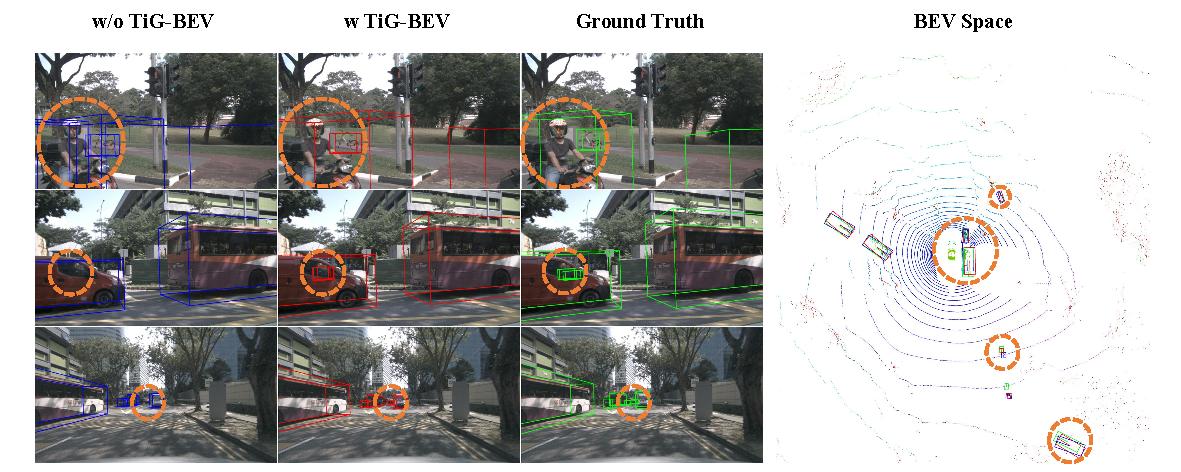
\includegraphics[scale=0.85]{cvpr_2022/det_result.pdf}
    \caption{\textbf{Visualization of Detection Results}. From left to right, we show the 3D object detection before and after the TiG-BEV learning schemes, ground-truth annotations, along with the overall BEV-space results.
    }
    \label{fig:aabb}
    %\hspace{-5cm}
\end{figure*}
\paragraph{Implementation Details.}
We implement our TiG-BEV using the BEVDet\cite{b19,b23} code base on 8 NVIDIA A100 GPUs, which is built on MMDetection3D toolkit\cite{b55}. A pre-trained CenterPoint~\cite{b53} with voxel size of $[0.1,0.1,0.2]$ is adopted as the LiDAR-based teacher, and the camera-based students include BEVDepth~\cite{b7}, BEVDet~\cite{b19} and BEVDet4D~\cite{b23}. During inference, the camare-based detecots only take multi-view images as input without the LiDAR data or teachers.
Referring to BEVDepth, we additionally add the dense depth supervision on top of BEVDet and BEVDet4D besides our TiG-BEV. We follow their official training configurations and hyperparameters as default, including data augmentation (random flip, scale and rotation), training schedule (2x), and others (AdamW optimizer~\cite{b16}, 2e-4 learning rate and batch size 8). For the main results on nuScenes val set in Table~\ref{tab:nus_val_sota}, we compare our TiG-BEV with all other methods under the CBGS strategy~\cite{b56}. For all other results, we do not utilize CBGS to better reveal the significance of proposed methods.

% Our TiG-BEV is trained for 2 × schedule 

% (20 epochs with CBGS strategy\cite{b56} or 24 epochs without CBGS strategy) with a batch size of 8 on 8 NVIDIA A100 GPUs. We use AdamW\cite{b16} optimizer with the initial learning rate of 2e-4, which drops at epoch 19 and 23 by a factor of 0.1 without CBGS strategy and drops at epoch 16 and 19 by a factor of 0.1 with CBGS strategy. In terms of data augmentation, the input images and points are randomly flipped, scaled and rotated. For the purpose of fair comparison, the above settings are aligned with mainstream methods. In ablation studies, we use BEVDepth\cite{b23} without CBGS strategy as our baseline.
%When we compare with other methods, we use BEVDet4d\cite{b23} with absolute depth supervision and CBGS strategy as our baseline. Otherwise, the results shown in tables, such as ablation studies, are taken from experiments without CBGS strategy.
%\begin{table}
% \vspace{-1.1cm}
\small
\centering

\begin{tabular}{L{4.0cm}|C{1.5cm}|C{1.5cm}|C{1.5cm}|C{1.5cm}}
\hline

\hline

\hline
Method  & Params  &FLOPs & Top1 & Latency\\
\hline

\hline
\hline
MobileNetV3-Small~\cite{howard2019searching}  & 2.9M & 0.1G & 67.4 & \textbf{5ms} \\
SeaFormer-T  & 1.8M & 0.1G & 67.9 & 7ms \\
\textbf{SeaFormer-T++}  & 1.9M & 0.1G & \textbf{69.8} & 7ms \\
\hline

\hline
\hline
MobileViT-XXS~\cite{mehta2021mobilevit}  & 1.3M & 0.4G & 69.0 & 24ms \\
MobileViTv2-0.50~\cite{mehta2022separable} & 1.4M & 0.5G & 70.2 & 32ms \\
MobileOne-S0*~\cite{vasu2022improved} & 2.1M & 0.3G & 71.4 & 14ms \\
MobileNetV2~\cite{sandler2018mobilenetv2} & 3.4M & 0.3G & 72.0 & 17ms \\
Mobile-Former96~\cite{chen2022mobile} & 4.8M & 0.1G & 72.8 & 31ms \\
SeaFormer-S & 4.1M & 0.2G & 73.3 & 12ms \\
\textbf{SeaFormer-S++} & 4.2M & 0.2G & \textbf{74.5} & \textbf{12ms} \\
\hline

\hline
\hline
EdgeViT-XXS~\cite{pan2022edgevits} & 4.1M & 0.6G & 74.4  & 71ms \\
LVT~\cite{yang2022lite} & 5.5M & 0.9G & 74.8 & 97ms \\
MobileViT-XS~\cite{mehta2021mobilevit} & 2.3M & 0.9G & 74.8 & 54ms \\
MobileNetV3-Large~\cite{howard2019searching} & 5.4M & 0.2G & 75.2 & \textbf{16ms} \\
Mobile-Former151~\cite{chen2022mobile} & 7.7M & 0.2G & 75.2 & 42ms \\
MobileViTv2-0.75~\cite{mehta2022separable} & 2.9M & 1.0G & 75.6 & 68ms \\
MobileOne-S1*~\cite{vasu2022improved} & 4.8M & 0.8G & 75.9 & 40ms \\
SeaFormer-B & 8.7M & 0.3G & 76.0 & 20ms \\
\textbf{SeaFormer-B++} & 8.8M & 0.3G & \textbf{77.0} & 20ms \\
\hline

\hline
\hline
MobileOne-S2*~\cite{vasu2022improved} & 7.8M & 1.3G & 77.4 & 63ms \\
EdgeViT-XS~\cite{pan2022edgevits} & 6.8M & 1.1G & 77.5  & 124ms \\
MobileViTv2-1.00~\cite{mehta2022separable} & 4.9M & 1.8G & 78.1 & 115ms \\
MobileOne-S3*~\cite{vasu2022improved} & 10.1M & 1.9G & 78.1 & 91ms \\
MobileViT-S~\cite{mehta2021mobilevit} & 5.6M & 1.8G & 78.4 & 88ms \\
EfficientNet-B1~\cite{tan2019efficientnet} & 7.8M & 0.7G & 79.1 & 61ms \\
EfficientFormer-L1~\cite{li2022efficientformer} & 12.3M & 1.3G & 79.2 & 94ms \\
Mobile-Former508~\cite{chen2022mobile}  & 14.8M & 0.5G & 79.3 & 102ms \\
MobileOne-S4*~\cite{vasu2022improved} & 14.8M & 3.0G & 79.4 & 143ms \\
SeaFormer-L & 14.0M & 1.2G & 79.9 & 61ms \\ 
\textbf{SeaFormer-L++} & 14.1M & 1.2G & \textbf{80.6} & \textbf{61}ms \\ 
\hline

\hline

\hline
\end{tabular}
\caption{Image classification results on ImageNet-1K \textit{val} set. The FLOPs and latency are measured with input size 224×224, except for MobileViT and MobileViTv2 that are measured with 256×256 according to their original implementations. * indicates re-parameterized variants~\cite{vasu2022improved}. The latency is measured on a single Qualcomm Snapdragon 865, and only an ARM CPU core is used for speed testing. No other means of acceleration, e.g., GPU or quantification, is used.}
\label{imagenet_table}
% \vspace{-2.2cm}
\end{table}
%\vspace{-2mm}

%\begin{figure}[t]
%  \centering 
%    \subfloat[\label{fig:a}]{
%		\includegraphics[scale=0.1]{cvpr_2022/result_before.jpg}}
%    \subfloat[\label{fig:b}]{
%		\includegraphics[scale=0.1]{cvpr_2022/result_after.jpg}}
%    \vspace{-3mm}
%  \caption{\textbf{Visualization of the detection results}. We show the results of detection \textbf{(a) before} and \textbf{(b) after} distillation with our method, the colors of prediction and ground truth are in yellow and blue, respectively.}
%  \label{fig:vis_compare}
%  \vspace{-3mm}
%\end{figure}










\subsection{Main Results}
%\vspace{-2mm}
\paragraph{On nuScenes Val Set.} 
In Table~\ref{tab:nus_val_sota}, we compare our TiG-BEV with other 3D object detectors on nuScenes val set. 
%We take BEVDet4d-R101\cite{b23} model with absolute depth supervision as baseline and 
As shown, our LiDAR-to-camera learning schemes respectively boost the three baseline models, BEVDet, BEVDet4D, and BEVDepth, by +3.2\%, +2.6\%, and +2.3\% NDS. This clearly demonstrates the significance of our TiG-BEV to improve the detection performance of multi-view BEV 3D object detection.

\begin{table}[t!]
    \centering
    \caption{\textbf{Ablation Study of Target Inner-geometry Learning. }$\mathcal{L}^R_{\rm{depth}}$ and $\mathcal{L}_{\rm{bev}}$  denote the losses of inner-depth supervision and inner-feature BEV distillation, respectively.}
    %\vspace{-2mm}
    \resizebox{1\columnwidth}{!}
    {\tablestyle{15pt}{1.0}
    \begin{tabular}{cc|cc}
    \toprule[1.2pt]
          $\mathcal{L}^R_{\rm{depth}}$&$\mathcal{L}_{\rm{bev}}$& mAP&NDS  \\
          \midrule
                        &           & 0.329         & 0.431 \\ 
             \checkmark &           & 0.339         & 0.440 \\
                        &\checkmark & 0.359         & 0.454 \\
              \checkmark&\checkmark & \textbf{0.366}         & \textbf{0.461} \\
    \bottomrule[1.2pt]
    \end{tabular}}
    \label{tab:main_ablation}
    %\vspace{-3mm}
\end{table}

\paragraph{Without CBGS~\cite{b56} Strategy.} 
In Table~\ref{tab:aaaa}, we present the results of TiG-BEV without the CBGS training strategy. Without the resampling of training data, the performance improvement of learning target inner-geometry becomes more notable, \textbf{+10.3\%, +7.3\%,} and \textbf{+3.7\%} mAP for the three baselines, which indicates the superior LiDAR-to-camera knowledge transfer of our TiG-BEV.



\paragraph{Comparison with BEVDistill~\cite{b9}.} 
In Table~\ref{cccc}, we compare our TiG-BEV with another LiDAR-to-camera learning method BEVDistill in the same setting. As shown, on top of a better baseline model, our approach can achieve higher performance boost for both mAP and NDS. This well demonstrates the superiority of target inner-geometry learning to BEVDistill's foreground-guided dense distillation.

% our TiG-BEV addresses such mismatch of cross-modal features, then achieves 2.3\% mAP and 2.0\% NDS gains than the heavy baseline. We also compare our method with other camera-only methods, our baseline can outperform the mainstream 3D object detection models through TiG-BEV. 
%What's more, there is an interesting finding that when we use ResNet18 as image backbone and after our distillation method, the model performance can be close to BEVDepth-R50.


% achieves 69.21\%, which is higher comparing to ResNet110. In particular, distilling }
% We observe that in some comparison methods, when ResNet20 is the student, ResNet56, though less powerful, is a better teacher than ResNet110. 
% What's worse, FitNet even deteriorated the performance of ResNet20 under the guidance of ResNet110. This phenomenon means the issue of capacities mismatch between inferior network and large network. 
% It also demonstrates that the target-aware transformer is more effective than trying to manually establish the links between student and teacher by spatial order.

%In the experiment, we compare different implementations of the target-aware transformer module. We found that setting $\theta(\cdot)$ as an identical function achieves the best performance. \KY{should we move this to the ablation study?} 
%We also report the result of setting $\theta(\cdot)$ as $1\times1$ convolution$+$BN in the ablation study. 
%\vspace{-1mm}
\begin{table}[t!]
    \centering
    \caption{\textbf{Ablation Study of Inner-depth Supervision.} We compare different settings for relative depth value calculation and depth reference selection. * denotes our implementation.}
    %\vspace{-2mm}
    \resizebox{1\columnwidth}{!}
    {\tablestyle{7pt}{1.0}
    \begin{tabular}{c|c|cc}
    \toprule[1.2pt]
          Setting &Depth Reference & mAP&NDS  \\
          \midrule
          BEVDepth$^*$ & - & 0.329 & 0.431 \\
          \midrule
        \multirow{2}{*}{All-to-Certain}& 3D Center  & 0.358         & 0.452 \\ 
             &2D Center  & 0.358        & 0.452 \\
             \midrule
             One-to-One &Each Pair & 0.360     & 0.458 \\
             \midrule
         \multirow{2}{*}{All-to-Adaptive}&Highest Conf & 0.357         & 0.455 \\
              
              &Smallest Error & \textbf{0.366}         & \textbf{0.461} \\
    \bottomrule[1.2pt]
    \end{tabular}}
    \label{tab:relative_ablation}
    %\vspace{-3mm}
\end{table}

\begin{table*}[ht]
\centering
\caption{\textbf{Ablation Study of 2D Backbones and Temporal Information.} CenterPoint~\cite{b53} and BEVDepth~\cite{b7} are adopted as the teacher and student models, respectively.}
\resizebox{2\columnwidth}{!}
{\tablestyle{12pt}{1}
\begin{tabular}{c|c|c|c|cc}
\toprule[1.2pt]
          Backbone&Resolution&Multi-frame&Method& mAP&NDS  \\
          \midrule
          VoxelNet & - & \checkmark&Teacher & 0.564 & 0.646 \\\midrule
          \multirow{4}{*}{ResNet-18}&\multirow{4}{*}{$256\times 704$}&\multirow{2}{*}{\checkmark}&Student & 0.285 & 0.405 \\ 
              & & &  + TiG-BEV& \textbf{0.323 (\textcolor{blue}{+3.8\%})}         & \textbf{0.430 (\textcolor{blue}{+2.5\%})} \\
              \cmidrule(lr){3-6}
                & & &  Student& 0.260  & 0.295 \\
               & & &    + TiG-BEV& \textbf{0.294 (\textcolor{blue}{+3.4\%})}  & \textbf{0.335 (\textcolor{blue}{+4.0\%})}\\
          \midrule
         \multirow{4}{*}{ResNet-50}&\multirow{4}{*}{$256\times 704$}&\multirow{2}{*}{\checkmark}&Student & 0.329 & 0.431 \\ 
              & & &    + TiG-BEV& \textbf{0.366 (\textcolor{blue}{+3.7\%})}         & \textbf{0.461 (\textcolor{blue}{+3.0\%})} \\
              \cmidrule(lr){3-6}
              
              & & &  Student& 0.298  & 0.328 \\
               & & &  + TiG-BEV& \textbf{0.338 (\textcolor{blue}{+4.0\%})}  & \textbf{0.375 (\textcolor{blue}{+4.7\%})}\\
          \midrule
          \multirow{4}{*}{ResNet-101}&\multirow{4}{*}{$512\times 1408$}&\multirow{2}{*}{\checkmark}&Student & 0.393 & 0.487 \\ 
              & & &  + TiG-BEV& \textbf{0.430 (\textcolor{blue}{+3.7\%})}         & \textbf{0.514 (\textcolor{blue}{+2.7\%})} \\
              \cmidrule(lr){3-6}
              & & &  Student& 0.345 & 0.366 \\
               & & &    + TiG-BEV& \textbf{0.403 (\textcolor{blue}{+5.8\%})}        & \textbf{0.416 (\textcolor{blue}{+5.0\%)}} 
         \\
               \bottomrule[1.2pt]
    \end{tabular}}
    \label{tab:many_ablation}
\end{table*}


\paragraph{Visualization.} 
As visualized in Figure~\ref{fig:aabb}, we show the detection results of BEVDepth before and after TiG-BEV, and the ground-truth annotations. We can clearly observe that more accurate results are obtained by our inner-geometry learning. Specifically, within the orange circles, the detection of false positives and ghosting objects can be reduced, and some 3D locations and orientations of the bounding boxes are also refined.
%\input{cvpr_2022/tex/tables/segmentation}

%\input{cvpr_2022/tex/tables/sgementation_coco}
%\vspace{-1mm}



%\input{cvpr_2022/tex/tables/cifar100-paramentric}





\subsection{Ablation Study}
\label{sec:ablation}
Here, we provide detailed experiments to validate the effectiveness of our approach from each of its components. We adopt BEVDepth as the student model by default.

\begin{figure}[t]
% \vspace{-0.5cm}
    \centering
    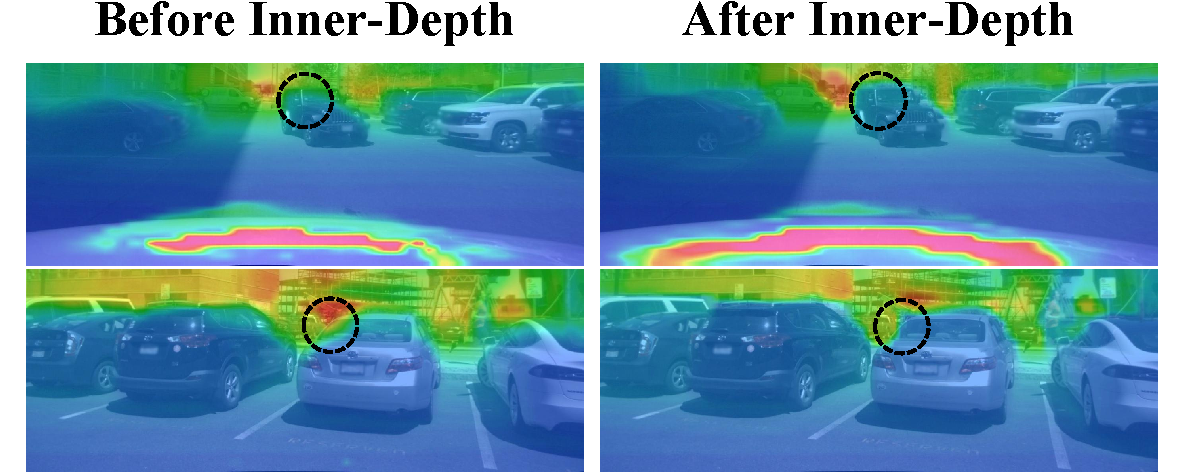
\includegraphics[scale=0.4]{cvpr_2022/ref_vis.pdf}
    \caption{\textbf{Visualization of Predicted Depth Maps,} which are before and after the inner-depth supervision, respectively.}
    \label{fig:ref_compare}
    %\hspace{-5cm}
\end{figure}

\paragraph{Inner-geometry Learning.} 
%\KY{find a better name}
The individual effectiveness of the two main components can be examined by only equipping one of them. We first study the impact of the inner-depth supervision. As shown in Table~\ref{tab:main_ablation}, we only introduce the inner-depth supervision to the vanilla baseline, i.e., BEVDepth, by which its mAP improves from 32.9\% to 33.9\% with a +1.0\% gain and its NDS reaches 44.0\% from 43.1\% with a +0.9\% gain. 
Instead, when we only use the inner-feature BEV distillation, the mAP boosts from 32.9\% to 35.9\% with a +3.0\% improvement and the NDS boosts from 43.1\% to 45.4\% with a +2.3\% improvement. In addition, the combination of both components achieves better +3.7\% mAP and +2.7\% NDS, demonstrating that the two proposed objectives might be complementary.

%\begin{figure} [t]
%    \centering 
%    \subfloat[\label{fig:a}]{
%		\includegraphics[scale=0.13]{cvpr_2022/relative_vis_before.png}}
%    \subfloat[\label{fig:b}]{
%		\includegraphics[scale=0.13]{cvpr_2022/relative_vis_after.png}}
%    \vspace{-3mm}
%    \caption{\textbf{The visualization of depth distribution.} (a) shows the origin predicted depth distribution of each valid pixel where exists projectable lidar points, while the depth distribution in (b) is predicted after inner relative depth supervision. The horizontal axis represents the discrete depth $\mathcal{D}_{\rm{i}}$ within the range of $\mathcal{[}0\mathcal{,}\mathcal{D}_{\rm{max}}\mathcal{]}$. The yellow pillar refers to the ground truth of depth and the red pillar refers to the predict depth whose height indicates the probability of the corresponding depth. The most obvious difference is marked in blue boxes.} 
%    \label{fig:imgnet_sigma} 
%    \vspace{-3mm}
%\end{figure}





%\begin{table}[t!]
%    \centering
%    \caption{\textbf{Ablation Study of Distillation.}  }
%    \vspace{-2mm}
%    \resizebox{1\columnwidth}{!}
%    {\tablestyle{20pt}{0.8}
%    \begin{tabular}{c|c|c}
%    \toprule
%          Methods& mAP&NDS  \\
%          \midrule
%                        Dense Feature Mimic  & 0.338         & 0.434 \\ 
%             Soft Foreground Feature Mimic  & 0.328        & 0.427 \\
%             Ours & \textbf{0.366}         & \textbf{0.458} \\
%    \bottomrule
%    \end{tabular}}
%    \label{tab:distill_ablation}
%    \vspace{-3mm}
%\end{table}


%We are also interested in that if the learning target (\ie teacher feature) is fixed, can the student adapt itself through target-aware transformer better? We compare different settings of $\theta(\cdot)$ including identical mapping against Conv$+$BN. The result on Cifar100 is presented on Table \ref{tab:cifar_1x1}. Surprisingly, the identical mapping for $\theta(\cdot)$ always performs better. 

%We further investigate the non-parametric implementation by setting both $\theta(\cdot)$ and $\gamma(\cdot)$ as identical mapping on ImageNet (Table~\ref{tab:non-parametric_imagenet}). The result shows that the semi-parametric version performs best, where the fixed teacher and the linear transformation applying to student feature can facilitate the student to reconfigure itself.



\begin{table}[t!]
    \centering
    \caption{\textbf{Ablation Study of Inner-feature BEV Distillation.} $\mathcal{L}^{IC}_{\rm{bev}}$ and $\mathcal{L}^{IK}_{\rm{bev}}$ denote the losses of inter-channel and inter-keypoint distillation, respectively.}
    %\vspace{-2mm}
    \resizebox{1\columnwidth}{!}
    {\tablestyle{15pt}{1.0}
    \begin{tabular}{cc|cc}
    \toprule[1.2pt]
          $\mathcal{L}^{IC}_{\rm{bev}}$&$\mathcal{L}^{IK}_{\rm{bev}}$& mAP&NDS  \\
          \midrule
                        &           & 0.329         & 0.431 \\ 
             \checkmark &           & 0.342         & 0.444 \\
                        &\checkmark & 0.358         & 0.452 \\
              \checkmark&\checkmark & \textbf{0.366}         & \textbf{0.461} \\
    \bottomrule[1.2pt]
    \end{tabular}}
    \label{tab:saf_ablation}
    %\vspace{-3mm}
\end{table}

\paragraph{Inner-depth Supervision.}
To calculate the relative depth values within foreground targets, we compare several methods concerning the relationships among different inner points, which can be divided into three paradigms, 1) \emph{All-to-Certain} calculates the relative depth from all sampled points to a certain reference point, such as the projected center of 3D bounding box or the center of 2D bounding box. 2) \emph{All-to-Adaptive} sets the reference depth in a dynamic manner, which selects the reference pixel with the highest confidence across all depth bins or the smallest depth error to the ground truth (Ours). 3) \emph{One-to-One} calculates the relative depth from each two sampled point pair. As shown in Table~\ref{tab:relative_ablation}, compared with other patterns, our \emph{All-to-Adaptive} with smallest depth errors obtains the best performance improvement, which indicates the dynamic depth reference point can flexibly adapt to different targets for inner-geometry learning. What's more, we visualize our depth prediction with and without the inner-depth supervision in Figure~\ref{fig:ref_compare}, which effectively refines the contours and edges of foreground objects.


\paragraph{Inner-feature BEV Distillation.}
Our TiG-BEV explores the BEV feature distillation from two perspectives, inter-channel and inter-keypoint. To validate their effectiveness, we also equip the model with one of them at a time and report the results in Table~\ref{tab:saf_ablation}. As shown, both inter-channel and inter-keypoint distillation contribute to the final performance, respectively boosting the NDS by +1.3\% and +2.1\%. This well illustrates the importance of learning inner-geometry semantics within different foreground targets in BEV space. Further combining them two can benefit the performance by +3.7\% and +3.0\% for mAP and NDS.

\paragraph{2D Backbones and Temporal Information.}
We further explore the influence of 2D backbones and temporal information to our TiG-BEV in Table~\ref{tab:many_ablation}. We observe that our TiG-BEV brings significant performance improvement consistent over different 2D backbones. Also, our target inner-geometry learning schemes can provide positive effect for both single-frame and multi-frame settings. The improvement of mAP ranges from \textbf{+3.4\%} to \textbf{+5.8\%} and the improvement of NDS ranges from \textbf{+2.5\%} to \textbf{+5.0\%}.



%We also conduct the thorough experiments to understand the contribution brought by the proposed patch-group distillation $\mathcal{L}_{\rm{TaT}}^{\mathcal{P}}$ and anchor-point distillation $\mathcal{L}_{\rm{TaT}}^{\mathcal{A}}$. As discussed previously, $\mathcal{L}_{\rm{TaT}}^{\mathcal{A}}$ is proposed to learn the global representation to capture long-range dependency while $\mathcal{L}_{\rm{TaT}}^{\mathcal{P}}$ is designed to concentrate on local feature. 
%By covering each one of them, the individual effectiveness of the two components can be examined.  
%As shown in Table. \ref{tab:main_ablation}, both objectives can improve the vanilla student significantly while $\mathcal{L}_{\rm{TaT}}^{\mathcal{P}}$ presents more efficacy. 
%The combination of both components achieves the best performance, demonstrating that the two proposed objectives are complementary.  

% Then, we give more insight with respect to the proposed objectives' functionality through sensitivity analysis. Specifically, we investigate the hyper-parameters that would influence the behaviour of the training process. In terms of the anchor-point distillation, this work utilizes average pooling to extract the anchor in a local area from the original feature, forming the associated anchor-point feature. It is a trade-off between noise reduction and representation preservation since bigger kernel would filter more noise along with more informative representation. Thus we study the sampling range (i.e. kernel size) that directly yields different feature resolution. Specially, when the $1\times 1$ pooling kernel is used, it degrades to the circumstance discussed in Sec. \ref{sec:formulation} and returns the original feature.
% The result exhibited in Table \ref{tab:anchor} supports our hypothesis that the full-size feature deteriorates the performance due to noise interference and presents poor performance compared to the other anchor-point features of smaller size. On the other hand, excessive sampling range would omit useful and informative representation and damage the performance.



% \mypara{Extra Width.}
% Then, we give more insight concerning the proposed extra width's functionality through ablation study. Specifically, we suppose that introducing extra width for ground truth bounding box before grid sampling would allow the distillation process to focus more on the edge information of foreground objects. 



%So we varied the value of the extra width by 0, 1, 2, 3 unit while keeping the other variables consistent, the length of an unit is equal to the width of a bev grid. 
%It is a trade-off between reducing computation overhead and summarizing fine-grained spatial information since a bigger kernel would reduce feature size along with more informative representation, \eg, when feature map size is reduced to $1 \times 1$, it degrades to ignoring the spatial information and posing one-to-one fashion distillation.
%Thus we study the pooling kernel size that directly yields different feature resolutions.
% Especially, when the $1\times 1$ pooling kernel is used, it degrades to the circumstance discussed in Section \ref{sec:formulation} and returns the original feature.
%The result exhibited in Table \ref{tab:anchor} supports our hypothesis that the full-size feature deteriorates the performance due to inferior capacity of student network and presents poor performance compared to the other anchor-point features of smaller size. On the other hand, excessive sampling range would omit useful and informative representation and damage the performance.
% The result exhibited in Table \ref{tab:comb_ablation} shows that when the extra width exists, our approach can further enhance the mAP. 

%Next we analyze the roi grid size used in grid sampling, the key factor of our inner-feature bev distillation.In Table \ref{tab:comb_ablation}, we found that generally, larger grid size is advantageous to our distillation, however we should make a trade-off because of the decreasing marginal gains. Overall, we found that the combination of $24\times 24$ grid size and using extra width can reach the best performance.
%however overlarge grid size may be unfavourable and we should make a trade-off between reducing computation overhead and extracting fine-grained spatial information since a $N\times N$ grid size results in $(N\times N)\times(N\times N)$ feature supervision. In our ablation study, we found that the combination of $24\times 24$ grid size and 2 unit extra width can reach the best performance.
%On the other hand, excessive extra width would lead to inadequate foreground structure supervision which will damage the performance.
%\begin{table}[t!]
%    \centering
%    \caption{\textbf{Ablation Study of Extra Width.} }
%    \vspace{-3mm}
%    \resizebox{1\columnwidth}{!}
%    {\tablestyle{10pt}{1}
%    \begin{tabular}{@{}l|ccccc@{}} 
%    \toprule
%         Extra width &0 &1 &2 &3    \\
%         \midrule
%         mAP &0.326 &\textbf{0.336} &0.335 &0.331\\
%         NDS &0.369 &\textbf{0.372} &0.364 &0.363 \\
%    \bottomrule
%    \end{tabular}
%    \label{tab:extra_width}}
%\vspace{-3mm}
%\end{table}

%\begin{table}[t!]
%    \centering
%    \caption{\textbf{Ablation Study of ROI Grid Size.}}
%    \vspace{-3mm}
%    \resizebox{1\columnwidth}{!}
%    {\tablestyle{10pt}{1}
%    \begin{tabular}{@{}l|cccc@{}}
%    \toprule
%         Grid size &$8\times 8$ &$16\times 16$&$24\times 24$&$32\times 32$ \\
%         \midrule
%        mAP &0.331 &0.335   &\textbf{0.338} & 0.333 \\
%        NDS &0.357 &0.364   &\textbf{0.375} & 0.354 \\
%    \bottomrule
%    \end{tabular}
%    \label{tab:grid_size}}
%    \vspace{-3mm}
%\end{table}








%\mypara{Ablation Study of ROI Grid Size.}
%Next we analyze a key factor of our structured attention feature supervision, the roi grid size used in grid sampling. In Table \ref{tab:comb_ablation}, we found that generally, larger grid size is advantageous to our distillation, however overlarge grid size may be unfavourable and we should make a trade-off between reducing computation overhead and extracting fine-grained spatial information since a $N\times N$ grid size results in $(N\times N)\times(N\times N)$ feature supervision. In our ablation study, we found that the combination of $24\times 24$ grid size and 2 unit extra width can reach the best performance.



% \begin{table}[t!]
% \centering
%     \caption{\textbf{Ablation Study of Extra Width.}}
%     %\vspace{-2mm}
%     \resizebox{1\columnwidth}{!}
%     {\tablestyle{25pt}{1.0}
%     \begin{tabular}{c|c|c}
%     \toprule[1.2pt]
%           Extra Width&mAP&NDS  \\
%           \midrule
%           &0.360       &  0.457     \\
%           %\midrule
%           \checkmark&  \textbf{0.366}      & \textbf{0.461}      \\
              
%     \bottomrule[1.2pt]
%     \end{tabular}}
%     \label{tab:comb_ablation}
%     %\vspace{-5mm}
% \end{table}

\iffalse
\begin{table}[t!]
\centering
    \caption{\textbf{Ablation Study of Different Combination of Extra Width and Grid Size.}}
    %\vspace{-2mm}
    \resizebox{1\columnwidth}{!}
    {\tablestyle{25pt}{0.8}
    \begin{tabular}{c|c|c|c}
    \toprule[1.2pt]
          Extra Width&Grid Size&mAP&NDS  \\
          \midrule
          \multirow{3}{*}{}&$16\times 16$ & 0.359       &  0.459     \\
                                      &$24\times 24$ & 0.360       &  0.457     \\
                                      &$32\times 32$ & 0.361       &  0.458     \\
          \midrule
          \multirow{3}{*}{\checkmark}&$16\times 16$ & 0.362       & 0.458      \\
                                      &$24\times 24$ &  \textbf{0.366}      & \textbf{0.461}      \\
                                      &$32\times 32$ &  0.365      &  0.458     \\
              
    \bottomrule[1.2pt]
    \end{tabular}}
    \label{tab:comb_ablation}
    %\vspace{-5mm}
\end{table}
\fi


\iffalse
\begin{table}[t!]
\centering
    \caption{\textbf{Ablation Study of Different Combination of Extra Width and Grid Size.}}
    %\vspace{-2mm}
    \resizebox{1\columnwidth}{!}
    {\tablestyle{20pt}{0.8}
    \begin{tabular}{c|c|c|c}
    \toprule[1.2pt]
          Extra Width&Grid Size&mAP&NDS  \\
          \midrule
          \multirow{4}{*}{0}&$8\times 8$ & \textbf{0.333}  & \textbf{0.377} \\ 
                                      &$16\times 16$ & 0.326       &  0.369     \\
                                      &$24\times 24$ & 0.330       &  0.352     \\
                                      &$32\times 32$ & 0.325       &  0.350     \\
          \midrule
          \multirow{4}{*}{1}&$8\times 8$ & 0.334  & 0.363 \\ 
                                      &$16\times 16$ &  \textbf{0.336}      &  \textbf{0.372}     \\
                                      &$24\times 24$ &  0.335      &  0.364     \\
                                      &$32\times 32$ &  0.333      &  0.353     \\
          \midrule
          \multirow{4}{*}{2}&$8\times 8$ & 0.331  & 0.357 \\ 
                                      &$16\times 16$ & 0.335       & 0.364      \\
                                      &$24\times 24$ &  \textbf{0.338}      & \textbf{0.375}      \\
                                      &$32\times 32$ &  0.333      &  0.354     \\
          \midrule
          \multirow{4}{*}{3}&$8\times 8$ & 0.331 &0.357  \\ 
                                      &$16\times 16$ & 0.331       &  \textbf{0.363}     \\
                                      &$24\times 24$ & 0.333  & 0.361  \\
                                      &$32\times 32$ & \textbf{0.335}       &  0.358     \\

              
    \bottomrule[1.2pt]
    \end{tabular}}
    \label{tab:comb_ablation}
    %\vspace{-5mm}
\end{table}
\fi



\section{Conclusion}
In this paper, we propose a novel target inner-geometry learning framework that enables the camera-based detector to inherit the effective foreground geometric semantics from the LiDAR modality. We first introduce an inner-depth supervision with target-adaptive depth reference to help the student learn better local geometric structures. Then, we conduct inner-feature distillation in BEV space for both channel-wise and keypoint-wise, which contributes to high-level inner-geometry semantics learning from the LiDAR modality. Extensive experiments are implemented to illustrate the significance of TiG-BEV for multi-view BEV 3D object detection. For future works, we will focus on exploring multi-modal learning strategy that can boost both camera and LiDAR modalities for superior real-world perception.

% This work develops a framework for knowledge distillation through a target-aware transformation that enables the student to aggregate the useful semantic over itself to enhance the expressivity of each pixel, which allows the student to act as a whole to mimic the teacher rather than minimize each partial divergence in parallel.
% Our method is successfully extended to semantic segmentation by the proposed hierarchical distillation consisting of patch-group and anchor-point distillation, designed to focus on local feature and long-range dependency. We conduct thorough experiments to validate the effectiveness of the method and advance the state-of-the-art.

%\section{Discussion}
%\textbf{Potential negative societal impact.} Our method has no ethical risk on dataset usage and privacy violation as all the benchmarks are public and transparent.

%\textbf{Limitations.} There are some issues of interest that we would like to explore in the future: (1) Currently, we only select the last layer of the backbone network for distillation. It would be interesting to see the efficacy when multiple layers are get involved with distillation which has been explored by some works \cite{Zagoruyko2017PayingMA,chen2021distilling}. (2) Also, we didn't investigate the effectiveness on other applications like object detection, which may need to design the new objective to fit the nature of specific application. 

%%%%%%%%% REFERENCES
\clearpage
{\small
\bibliographystyle{ieee_fullname}
\bibliography{egbib}
}

\end{document}
